%% -----------------------------------------------------------
%% Projeto 1 da disciplina de INF2608 - Fundamentos de Computação Gráfica
%% Relatório LaTeX com corpo teórico e rastreabilidade consolidada.

\documentclass[portuguese]{sbcreviews-2025}%
\usepackage[misc,geometry]{ifsym}
\usepackage{aas_macros}
\usepackage[bottom]{footmisc}
\usepackage{tabularray}
\usepackage{afterpage}
\usepackage{url}
\usepackage{pifont}

\setcitestyle{square}
\captionsetup[figure]{hypcap=false}
\newcommand{\slidescite}[2]{\citep[pp.~#2]{#1}}
\newcommand{\pbrtcontentsurl}{https://pbr-book.org/4ed/contents.html}
\newcommand{\DeclarePBRTSectionURL}[2]{\expandafter\def\csname pbrturl@#1\endcsname{#2}}
\newcommand{\pbrtsectionurl}[1]{%
    \ifcsname pbrturl@#1\endcsname
        \csname pbrturl@#1\endcsname
    \else
        \pbrtcontentsurl
    \fi
}
\DeclarePBRTSectionURL{1.2}{https://pbr-book.org/4ed/Introduction/Photorealistic_Rendering_and_the_Ray-Tracing_Algorithm.html}
\DeclarePBRTSectionURL{3.5}{https://pbr-book.org/4ed/Geometry_and_Transformations/Normals.html}
\DeclarePBRTSectionURL{3.7}{https://pbr-book.org/4ed/Geometry_and_Transformations/Bounding_Boxes.html}
\DeclarePBRTSectionURL{5.2}{https://pbr-book.org/4ed/Cameras_and_Film/Projective_Camera_Models.html}
\DeclarePBRTSectionURL{7.3}{https://pbr-book.org/4ed/Primitives_and_Intersection_Acceleration/Bounding_Volume_Hierarchies.html}
\DeclarePBRTSectionURL{8.1}{https://pbr-book.org/4ed/Sampling_and_Reconstruction/Sampling_Theory.html}
\DeclarePBRTSectionURL{8.5}{https://pbr-book.org/4ed/Sampling_and_Reconstruction/Stratified_Sampler.html}
\DeclarePBRTSectionURL{9.3}{https://pbr-book.org/4ed/Reflection_Models/Specular_Reflection_and_Transmission.html}
\DeclarePBRTSectionURL{9.5}{https://pbr-book.org/4ed/Reflection_Models/Dielectric_BSDF.html}
\DeclarePBRTSectionURL{11.2}{https://pbr-book.org/4ed/Volume_Scattering/Transmittance.html}
\DeclarePBRTSectionURL{12.4}{https://pbr-book.org/4ed/Light_Sources/Area_Lights.html}
\newcommand{\pbrtbook}{\emph{Physically Based Rendering} (PBRT 4e)}
\newcommand{\pbrtsec}[1]{\citep[\href{\pbrtsectionurl{#1}}{Se\c{c}\~ao~#1}]{pharr2023pbrt}}
\newcommand{\pbrtsecpair}[2]{\citep[\href{\pbrtsectionurl{#1}}{Se\c{c}\~ao~#1} e \href{\pbrtsectionurl{#2}}{Se\c{c}\~ao~#2}]{pharr2023pbrt}}
\newcommand{\pbrtsecs}[1]{\citep[\href{\pbrtcontentsurl}{Se\c{c}\~oes~#1}]{pharr2023pbrt}}
\newcommand{\figcmd}[1]{%
    \par\medskip
    \begingroup
    \setlength{\fboxsep}{6pt}%
    \noindent\colorbox{black!5}{%
        \parbox{\dimexpr\linewidth-2\fboxsep\relax}{%
            \footnotesize\textbf{Comando gerador}\par
            \vspace{2pt}%
            {\footnotesize\raggedright\ttfamily\obeyspaces\detokenize{#1}\par}%
        }%
    }\par
    \endgroup
    \medskip
}

\definecolor{engtitle}{rgb}{0.5,0.5,0.5}
\definecolor{darkblue}{rgb}{0.0,0.0,0.0}
\hypersetup{colorlinks,breaklinks,
            linkcolor=darkblue,urlcolor=darkblue,
            anchorcolor=darkblue,citecolor=darkblue}
\emergencystretch=3em
\sloppy
\hbadness=10000
\vbadness=10000
\hfuzz=70pt
\vfuzz=2pt
\raggedbottom

\category{Projeto 1 da disciplina de INF2608\\Fundamentos de Computação Gráfica}
\title[Análise Técnico-Científica de Ray Tracing]{Análise Técnico-Científica\\de uma Implementação de Ray Tracing}
\engtitle{\textcolor{engtitle}{Technical-Scientific Analysis\\of a Ray Tracing Implementation}}

\author[Yang Ricardo Barcellos Miranda]{
\affil{\textbf{Yang Ricardo Barcellos Miranda}~[\href{mailto:ymiranda@inf.puc-rio.br}{\nolinkurl{ymiranda@inf.puc-rio.br}}]}
}

\institution{Pontifícia Universidade Católica do Rio de Janeiro - PUC-Rio}

\begin{document}
\begin{frontmatter}

\maketitle

\begin{abstract-pt}
Este artigo apresenta uma análise técnico-científica da implementação de ray tracing desenvolvida no Projeto 1 da disciplina de INF2608. O objetivo é verificar, a partir do código efetivamente executável, quais componentes geométricos, fotométricos e amostrais foram materializados, como eles se relacionam com os slides da disciplina e em que medida o resultado se aproxima de referências selecionadas de PBRT 4e. O texto enfatiza as explicações matemáticas sobre formação da imagem, interseções, iluminação local, amostragem, reflexão, refração e geometria triangular, e consolida a rastreabilidade detalhada em quadros finais de referência e evidência com notas sobre páginas dos slides e linhas de código.
\end{abstract-pt}

\begin{abstract-en}
This paper presents a technical-scientific analysis of the ray tracing implementation developed for the INF2608 course project. Its goal is to verify, from the executable code itself, which geometric, photometric, and sampling components were materialized, how they relate to the course slides, and to what extent the result aligns with selected PBRT 4e references. The text emphasizes the mathematical discussion of image formation, intersections, local illumination, sampling, reflection, refraction, and triangle geometry, and consolidates detailed traceability in final reference-and-evidence tables with notes pointing to slide pages and source-code lines.
\end{abstract-en}

\begin{pchaves}
traçado de raios, computação gráfica, PBRT, amostragem, BVH, renderização
\end{pchaves}

\begin{keywords}
ray tracing, computer graphics, PBRT, sampling, BVH, rendering
\end{keywords}

\begin{dates}
\noindent{\sffamily\textbf{Entrega:}} 10/05/2026
\end{dates}

\end{frontmatter}

\section{Introdução}
\label{sec:introducao-v3}

Este artigo analisa a implementação de ray tracing disponível no repositório do Projeto 1~\citep{inf2608projectrepo}. O foco principal é o código em \path{src/ray_tracing_2/}, lido em conjunto com os slides da disciplina, de autoria de Waldemar Celes~\citep{inf2608slides04,inf2608slides05,inf2608slides06}, e com referências selecionadas de \pbrtbook, em especial \pbrtsecs{1.2, 3.5, 3.7, 5.2, 7.3, 8.1, 8.5, 9.3, 9.5, 11.2 e 12.4}. A intenção não é recontar genericamente o que um ray tracer deveria fazer, mas entender o que esta base realmente entrega, quais escolhas de implementação sustentam cada efeito visual e em que pontos a teoria exigida pelo tema é maior do que a base atual tenta cobrir.

A organização do texto segue uma leitura mais próxima de engenharia de software do que de reconstrução teórica completa. Primeiro, o relatório observa o pipeline do traçador e a divisão de responsabilidades entre filme, câmera, cena, materiais e luzes. Depois, discute as extensões ópticas e amostrais, a geometria triangular e as estruturas de aceleração. As imagens principais ficam reunidas em uma seção específica de evidências visuais, na qual cada figura é acompanhada por uma leitura do que ela comprova, pelos metadados mais relevantes do render e pelo comando gerador correspondente.

Essa escolha de tom é intencional. O texto prioriza arquitetura, contratos entre módulos, reprodutibilidade e decisões de implementação, sem perder de vista a álgebra linear, a óptica geométrica e o cálculo que sustentam essas decisões. O objetivo não é substituir uma derivação teórica exaustiva, mas mobilizar a teoria necessária para explicar por que a base funciona, onde ela simplifica o problema e em que pontos um avanço posterior exigiria formalização mais forte. Para preservar a fluidez do corpo principal, a rastreabilidade detalhada aparece nos anexos finais. O Anexo A reúne quadros consolidados de \emph{conceitos de referência}, \emph{evidência principal} e \emph{nota}, em que as notas sintetizam as páginas dos slides, as seções mais próximas em PBRT e as linhas de código mais relevantes. O Anexo B mantém duas vistas complementares do diagrama de classes: uma versão inicial, mais sintética, e uma versão estendida que incorpora a infraestrutura experimental hoje presente na base.

\section{Núcleo Geométrico e Fotométrico do Traçador}
\label{sec:nucleo-v3}

\subsection{Pipeline geral do traçador}
\label{sec:pipeline-v3}

O pipeline do traçador pode ser lido como uma composição de quatro etapas. Primeiro, o filme define a amostragem do pixel; depois, a câmera converte a amostra em um raio primário; em seguida, a cena resolve a primeira interseção visível; por fim, o material associado ao \emph{hit}\footnote{Neste texto, \emph{hit} designa o registro da interseção válida selecionada pelo teste de visibilidade; \emph{closest hit} é a interseção com menor parâmetro positivo \(t\) ao longo do raio.} calcula a contribuição local e, quando necessário, dispara raios secundários. Em forma resumida, a cor do pixel pode ser entendida como

\[
C_{ij} = \frac{1}{N}\sum_{k=1}^{N} L\bigl(r_{ij,k}\bigr),
\]

em que cada raio \(r_{ij,k}\) nasce na câmera, atravessa a cena e devolve uma estimativa da radiância naquela direção. O caso básico do projeto usa \(N=1\) com uma amostra central; os casos com antialiasing substituem essa leitura pontual por uma média sobre o domínio do pixel.

Do ponto de vista arquitetural, esse encadeamento tem uma consequência importante: o núcleo do renderizador continua pequeno mesmo quando a ótica fica mais rica. \texttt{Film.render()} gera amostras, \texttt{Camera.generate\_ray()} produz raios, \texttt{Scene.compute\_intersection()} escolhe o \emph{closest hit} e \texttt{Scene.trace\_ray()} delega ao material a decisão de permanecer no sombreamento local ou seguir por recursão. Essa separação é central para entender por que reflexão, refração e transmitância puderam ser adicionadas sem substituir o pipeline original.

\subsection{Raio paramétrico, visibilidade e registro de interseção}
\label{sec:raio-v3}

O ponto de partida do Slide 4 é a modelagem do raio por

\[
\mathbf{r}(t)=\mathbf{o}+t\,\hat{\mathbf{d}},\qquad t\ge 0,
\]

em que \(\mathbf{o}\) é a origem, \(\hat{\mathbf{d}}\) é a direção normalizada e \(t\) parametriza a posição ao longo do feixe~\slidescite{inf2608slides04}{7--9}. Em óptica geométrica, essa escrita abstrai a propagação retilínea da luz em meios homogêneos; em computação gráfica, ela transforma visibilidade em busca do menor \(t>0\) compatível com uma superfície.

O repositório segue exatamente essa lógica. O raio é carregado por \texttt{Ray}; o registro da melhor interseção é encapsulado em \texttt{Hit}; e a cena trabalha com um único acumulador que preserva a interseção frontal mais próxima. A distinção entre \texttt{front\_face} e \texttt{backfacing}, calculada em \texttt{Hit.set\_face\_normal()}, começa como um detalhe geométrico de orientação de normal, mas depois se torna decisiva para os materiais refrativos, pois separa entrada e saída de meios diferentes.

\subsection{Interseções básicas e controle numérico de \texorpdfstring{$\varepsilon$}{epsilon}}
\label{sec:intersecoes-v3}

Nos slides, o plano é descrito pela equação implícita

\[
(\mathbf{x}-\mathbf{p}_0)\cdot\hat{\mathbf{n}}=0,
\]

e a substituição de \(\mathbf{r}(t)\) produz a solução linear

\[
t = \frac{(\mathbf{p}_0-\mathbf{o})\cdot\hat{\mathbf{n}}}{\hat{\mathbf{d}}\cdot\hat{\mathbf{n}}}.
\]

A esfera, por sua vez, impõe

\[
\lVert\mathbf{x}-\mathbf{c}\rVert^2-r^2=0,
\]

que, após substituição do raio, leva à quadrática \(at^2+bt+c=0\), cujo discriminante \(\Delta=b^2-4ac\) decide ausência, tangência ou dupla interseção~\slidescite{inf2608slides04}{10--18}. Em ambos os casos, o ponto relevante para a câmera é a menor raiz positiva.

O código espelha esse raciocínio em \texttt{Plane.intersect()} e \texttt{Sphere.intersect()}. Há também um segundo cuidado, menos visível na dedução analítica e muito importante na prática: a cena desloca a origem dos raios secundários por um pequeno \(\varepsilon\) ao longo da normal geométrica. Esse deslocamento evita auto-interseções espúrias em sombras, reflexão e refração, isto é, o clássico \emph{shadow acne}\footnote{Artefato numérico de auto-oclusão causado por reinterseção espúria do próprio ponto sombreado depois de erros de arredondamento em ponto flutuante.}. O ganho aqui não é conceitual, mas numérico: sem essa margem, a formulação teórica correta passa a falhar por erro de ponto flutuante.

\subsection{Câmera pinhole, filme e espaços de coordenadas}
\label{sec:camera-v3}

O Slide 4 reconstrói a câmera pinhole\footnote{Modelo ideal de formação de imagem em que todos os raios partem de um único centro ótico; por isso, não há abertura finita nem profundidade de campo.} por uma base ortonormal local e pela geometria do plano de imagem~\slidescite{inf2608slides04}{19--39}. Em termos algébricos, isso equivale a uma mudança de base entre espaço da câmera e espaço global. Se \(\theta\) é o campo de visão vertical e \(f\) a distância do pinhole ao plano de projeção, então a meia-altura do filme é dada por

\[
\Delta v = f\tan\left(\frac{\theta}{2}\right),
\qquad
\Delta u = \Delta v\,\frac{w}{h}.
\]

Na implementação, \texttt{Camera} usa \texttt{glm.lookAt()} para construir a transformação de visão e sua inversa, e \texttt{generate\_ray()} produz o raio primário a partir das coordenadas normalizadas do pixel. A formulação é de câmera pinhole pura: todos os raios partem de um único centro ótico. Isso significa que \texttt{focal\_distance} é distância geométrica ao plano de projeção, e não distância focal de lente fina nem parâmetro de profundidade de campo. Esse detalhe precisa ser explicitado no texto para que o leitor não projete sobre o código uma física óptica que ele não pretende resolver.

Do lado do filme, \texttt{get\_sample()} e \texttt{get\_samples\_for\_pixel()} deixam claro que o pixel é tratado como domínio de integração. A versão mais simples avalia uma única amostra central; a versão com supersampling\footnote{No contexto do projeto, \emph{supersampling} significa estimar a cor do pixel pela média de múltiplas amostras subpixel, e não por filtragem ótica da câmera.} transforma a formação da cor final em uma média sobre várias amostras. A câmera, portanto, fixa a geometria da imagem, enquanto o filme fixa a estratégia de amostragem dessa geometria.

\subsection{Phong, luz pontual, termo ambiente e sombras diretas}
\label{sec:phong-v3}

O fechamento do núcleo do traçador é o modelo local de Phong, expresso como soma de termo ambiente, componente difusa lambertiana e componente especular dependente do vetor refletido~\slidescite{inf2608slides04}{40--55}. Em forma resumida,

\[
L_o \approx k_a L_a + k_d L_i\max(0,\hat{\mathbf{n}}\cdot\hat{\mathbf{l}})
+ k_s L_i\max(0,\hat{\mathbf{r}}\cdot\hat{\mathbf{v}})^s.
\]

Fisicamente, trata-se de um modelo local e fenomenológico; computacionalmente, ele é suficiente para capturar a dependência angular da superfície sem resolver transporte global de energia. A sombra dura aparece como teste binário de visibilidade entre o ponto sombreado e a fonte.

\texttt{PhongMaterial.direct\_lighting()} implementa esse cálculo de forma direta: para cada luz, o código obtém radiância incidente e direção, soma a parcela difusa e a parcela especular, e combina o resultado com o termo ambiente. Já \texttt{Scene.transmittance()} generaliza o raio de sombra dos slides: para materiais opacos, ele se reduz ao caso binário; para materiais transparentes, ele passa a acumular transmitâncias ao longo do segmento até a fonte. Essa generalização pertence ao bloco mais avançado do projeto, mas sua raiz conceitual já está presente no núcleo do Slide 4.

Há ainda uma nuance importante de modelagem. A formulação didática clássica para fonte pontual costuma incluir decaimento geométrico por \(1/r^2\); nesta base, \texttt{PointLight} preserva a convenção simplificada do enunciado e trata \texttt{power} como radiância incidente constante. Não se trata de erro, mas de simplificação deliberada, pertinente ao contexto didático, e por isso a interpretação física dessa escolha precisa ser declarada explicitamente na seção de limites.

\section{Extensões Ópticas, Amostrais e de Transformação}
\label{sec:extensoes-v3}

\subsection{Antialiasing como integração estocástica sobre o pixel}
\label{sec:aa-v3}

O Slide 5 reinterpreta o pixel como um domínio de amostragem, e não como uma posição única~\slidescite{inf2608slides05}{4--8}. A consequência numérica é que a cor do pixel passa a ser estimada pela média de várias amostras de radiância,

\[
\hat L = \frac{1}{N}\sum_{k=1}^{N} L(x_k),
\]

convertendo aliasing estruturado em ruído de alta frequência. Na base atual, \texttt{film.py} opera com três regimes: \texttt{center}, \texttt{jittered} e \texttt{stratified}. A primeira escolha produz o baseline determinístico; as outras duas distribuem as amostras no interior do pixel. Após a refatoração da infraestrutura de amostragem, os padrões bidimensionais passaram a viver em \texttt{sampling.py}, o que torna a separação conceitual mais clara: o módulo de amostragem define padrões no quadrado unitário; o filme interpreta esses padrões como coordenadas físicas no pixel.

\subsection{Instanciação, coordenadas homogêneas e transformação de normais}
\label{sec:instancia-v3}

O bloco de transformações do Slide 5 introduz a ideia de instância geométrica: em vez de redefinir a interseção de cada forma transformada, o raio é levado para o espaço local da primitiva canônica~\slidescite{inf2608slides05}{9--13}. Em coordenadas homogêneas, isso significa aplicar a inversa da transformação ao raio incidente. Para as normais, porém, a transformação correta é a inversa transposta,

\[
\mathbf{n}' = (M^{-1})^{T}\mathbf{n},
\]

pois a normal deve permanecer ortogonal ao plano tangente após transformações afins gerais.

\texttt{Instance.intersect()} codifica exatamente esse fluxo. O raio entra no espaço local pela matriz inversa; a interseção é resolvida na forma base; a posição volta ao espaço global pela transformação direta; e a normal é convertida pela inversa transposta. O ponto matemático crucial é que aplicar \(M\) diretamente à normal preservaria a transformação de vetores tangentes, mas não a ortogonalidade da normal ao plano tangente quando há escala não uniforme. Essa é uma daquelas partes do projeto em que a álgebra linear deixa de ser apenas pano de fundo e passa a determinar a correção geométrica do resultado visual.

\subsection{Luz de área, integração sobre o emissor e penumbra}
\label{sec:arealight-v3}

Nos slides, a luz de área substitui a fonte pontual idealizada por um emissor com extensão geométrica finita~\slidescite{inf2608slides05}{14--23}. A penumbra surge porque diferentes sub-regiões da fonte são visíveis ou ocluídas de modo diferente a partir do ponto sombreado. Em termos numéricos, isso exige integrar a contribuição luminosa sobre a superfície emissiva.

\texttt{AreaLight.sample\_radiance()} aproxima essa integral por soma discreta sobre uma malha \texttt{samples\_u} \(\times\) \texttt{samples\_v}, com padrões \texttt{uniform}, \texttt{regular} e \texttt{stratified}. Diferentemente da \texttt{PointLight}, a fonte extensa introduz atenuação geométrica explícita com a distância e um termo angular de emissão. A implementação, portanto, preserva a convenção simplificada da luz pontual, mas adota uma leitura mais geométrica quando a fonte possui área. Essa dualidade precisa aparecer no texto porque ela tem efeito direto na interpretação física das imagens e impede tratar cenas mistas como se obedecessem a uma única convenção radiométrica rigorosa.

\subsection{De traçador local a traçador recursivo}
\label{sec:recursivo-v3}

O salto conceitual do Slide 5 é que o pipeline local do Slide 4 não é descartado; ele é reutilizado recursivamente~\slidescite{inf2608slides05}{26--35}. Em termos algorítmicos, alguns materiais deixam de devolver apenas uma cor local e passam a disparar novos raios. Para uma leitura mais orientada a engenharia, a principal mudança é esta: o material deixa de ser só uma função de cor local e passa a controlar continuidade de caminho e custo computacional, levando em consideração a profundidade da recursão da reflexão especular, transmissão especular e atenuação ao longo do trajeto.

Na base atual, \texttt{Scene.trace\_ray()} mantém-se intencionalmente enxuta: encontra o \emph{hit} mais próximo e delega a avaliação ao material. A profundidade é controlada por \texttt{Scene.can\_spawn\_ray()}, o que impõe um limite finito à recursão. Esse truncamento é necessário para conter o custo computacional e, ao mesmo tempo, coerente com a ideia de que contribuições sucessivas tendem a decair com a refletância ou a transmitância do material.

\subsection{Reflexão especular com Fresnel-Schlick}
\label{sec:fresnel-v3}

No bloco de reflexão, os slides introduzem a aproximação de Schlick\footnote{Aproximação polinomial de baixo custo para o termo de Fresnel, usada aqui para preservar a dependência angular da refletância sem resolver toda a ótica eletromagnética do problema.},

\[
R(\theta)=R_0 + (1-R_0)(1-\cos\theta)^5,
\]

como forma de baixo custo para modular a refletância com o ângulo de visão~\slidescite{inf2608slides05}{26--28}. Na implementação, \texttt{ReflectiveMaterial} reaproveita o sombreamento local de Phong e o pondera por \((1-R)\), enquanto a contribuição do raio refletido é ponderada por \(R\). O resultado é um material recursivo plausível e incrementalmente consistente com o restante do projeto, ainda que não equivalente a um BRDF\footnote{\emph{Bidirectional Reflectance Distribution Function}. O termo aparece aqui apenas como referência conceitual: a implementação preserva a dependência angular da refletância, mas não se propõe a cobrir um modelo fisicamente completo.} fisicamente completo.

\subsection{Refração dielétrica, Lei de Snell e Beer-Lambert}
\label{sec:refracao-v3}

O bloco de refração é o trecho matematicamente mais rico do projeto. A interface entre meios obedece à Lei de Snell,

\[
\eta_i\sin\theta_i = \eta_t\sin\theta_t,
\]

e a intensidade transmitida sofre atenuação com a distância percorrida no meio, segundo a Lei de Beer-Lambert\footnote{Modelo de absorção exponencial no meio, em que a transmitância decai com a distância percorrida e com o coeficiente de absorção.}. Na implementação, essa atenuação deve ser lida como aproximação para um dielétrico homogêneo em RGB, e não como integração volumétrica geral. A sequência efetiva do código é: calcular a fração refletida por Schlick, escolher a razão \(\eta_i/\eta_t\) com base na orientação da interface e, por fim, atenuar o raio transmitido conforme o comprimento percorrido no material.

\texttt{TransparentMaterial.eval()} codifica exatamente essa cadeia. A distinção entre \texttt{front\_face} e \texttt{backfacing} define se o raio entra ou sai do meio; \texttt{glm.refract()} produz a direção transmitida; e a reflexão interna total aparece quando a solução refratada se torna inviável. Na base atual, essa verificação ainda é mediada por um teste heurístico sobre a direção refratada, suficiente para as cenas do relatório, mas menos rigoroso do que uma formulação explícita a partir do radicando da Lei de Snell. Em paralelo, \texttt{TransparentMaterial.shadow\_transmittance()} aplica a atenuação de Beer-Lambert aos raios de sombra quando estes deixam o meio. O resultado é uma aproximação consistente para um dielétrico homogêneo em RGB, mas ainda distante de um tratamento espectral ou volumétrico completo.

\subsection{Da sombra binária à transmitância acumulada}
\label{sec:transmitancia-v3}

O caso mais elegante de reaproveitamento arquitetural no projeto é a generalização do raio de sombra. O que antes respondia apenas \emph{visível} ou \emph{ocluído} passa a acumular fatores multiplicativos ao atravessar materiais transparentes~\slidescite{inf2608slides05}{33--35},

\[
T = \prod_k a_k^{s_k}.
\]

Em termos computacionais, \texttt{Scene.transmittance()} percorre o segmento até a fonte, interrompe quando encontra um material opaco e, para materiais transparentes, delega ao método \texttt{shadow\_transmittance()} a atualização do throughput\footnote{Aqui, \emph{throughput} significa o fator multiplicativo acumulado ao longo do caminho de sombra, e não um fluxo radiométrico absoluto.}. Esse desenho mostra que o projeto não criou um caminho paralelo para transparência; ele estendeu o mecanismo de visibilidade já existente.

\section{Triângulos e Estruturas de Aceleração}
\label{sec:triangulos-v3}

\subsection{Triângulo, área orientada e coordenadas baricêntricas}
\label{sec:tri-bar-v3}

O Slide 6 começa pelo triângulo como primitiva elementar de malhas~\slidescite{inf2608slides06}{3--4}. Com vértices \(\mathbf{a}\), \(\mathbf{b}\) e \(\mathbf{c}\), os vetores de aresta

\[
\mathbf{e}_1 = \mathbf{b}-\mathbf{a},
\qquad
\mathbf{e}_2 = \mathbf{c}-\mathbf{a}
\]

definem uma área orientada

\[
A = \frac{\lVert \mathbf{e}_1 \times \mathbf{e}_2 \rVert}{2},
\]

enquanto qualquer ponto interno pode ser descrito por coordenadas baricêntricas,

\[
\mathbf{p}=\mathbf{a}+u\mathbf{e}_1+v\mathbf{e}_2,
\qquad
u\ge 0,\ v\ge 0,\ u+v\le 1.
\]

Na base atual, \texttt{Triangle} pré-computa \texttt{e1}, \texttt{e2} e a normal geométrica orientada por produto vetorial. Triângulos degenerados são rejeitados já na construção da forma, o que evita que a malha carregue primitivas nulas para o estágio de interseção.

\subsection{Interseção raio-triângulo por Möller-Trumbore}
\label{sec:moller-v3}

O coração algébrico do Slide 6 é o teste de Möller-Trumbore\footnote{Algoritmo direto para interseção raio-triângulo que resolve \(t\), \(u\) e \(v\) sem construir explicitamente a equação do plano do triângulo.}. Em forma compacta, ele resolve a igualdade

\[
\mathbf{o}+t\hat{\mathbf{d}} = \mathbf{a}+u\mathbf{e}_1+v\mathbf{e}_2,
\]

sem construir explicitamente o plano do triângulo. A solução só é válida se \(u\ge 0\), \(v\ge 0\), \(u+v\le 1\) e \(t>0\). \texttt{Triangle.intersect()} implementa exatamente essa forma operacional por meio de \texttt{pvec}, \texttt{det}, \texttt{u}, \texttt{v}, \texttt{qvec} e \texttt{t\_candidate}. O teste para \texttt{abs(det) < eps} cobre o caso de quase paralelismo entre o raio e o plano do triângulo.

\subsection{Malha triangulada e BVH local}
\label{sec:mesh-bvh-v3}

Os slides passam do triângulo isolado para a malha e, em seguida, para estruturas de aceleração~\slidescite{inf2608slides06}{13--36}. O repositório segue esse mesmo encadeamento. \texttt{TriangleMesh} pode ser construído a partir de listas de vértices e faces e participa do mesmo pipeline de interseção, material e iluminação das primitivas analíticas. Quando a malha ativa sua BVH local, caixas AABB\footnote{\emph{Axis-Aligned Bounding Boxes}: volumes de contenção alinhados aos eixos cartesianos, usados aqui para poda espacial local.} passam a funcionar como volumes de contenção, e a travessia recursiva decide em que subárvores vale a pena continuar.

O ponto mais importante aqui é o alcance da aceleração. A base reúne uma BVH estática por malha, construída por mediana em eixo dominante, mas não um acelerador global da cena. Em consequência, a redução de custo aparece dentro da \texttt{TriangleMesh}; o topo da cena continua a ser percorrido de forma sequencial por \texttt{Scene.compute\_intersection()}.

\section{Evidências Visuais e Leitura das Figuras}
\label{sec:evidencias-v3}

As figuras desta seção usam cenas dedicadas do projeto e algumas extensões selecionadas. O objetivo não é substituir a análise teórica desenvolvida nas seções precedentes, mas oferecer evidência visual organizada do que ela descreve. Em cada caso, a pergunta orientadora é a mesma: o que exatamente a figura mostra, qual comando a reproduz e que hipótese técnica ela ajuda a sustentar. Para preservar a legibilidade no corpo em duas colunas, as imagens ficam contidas na largura da coluna; as versões ampliadas das mesmas evidências aparecem no Anexo C.

\subsection{CLI, snapshots e estimativa como infraestrutura experimental}
\label{sec:infra-exp-v3}

Antes da leitura figura a figura, vale explicitar que os comandos impressos sob cada imagem não são ornamentos editoriais. A camada de CLI centraliza, em \texttt{CommonRenderOptions}, os parâmetros que de fato definem o experimento -- resolução, \texttt{spp}, \texttt{sampling\_mode}, semente e calibração -- e impõe um contrato estável aos diferentes \emph{entrypoints}. Isso importa metodologicamente porque evita que comparações entre \texttt{req2}, \texttt{req4}, \texttt{proj1\_final} e \texttt{proj1\_final\_v2} misturem diferença de cena com diferença de interface de execução.

Essa padronização é complementada por snapshots persistentes e por uma estimativa calibrável de custo. \texttt{RenderSnapshot.from\_runtime()} registra configuração de imagem, câmera, cena, objetos e luzes em \texttt{properties.json} e \texttt{properties.md}, enquanto \texttt{RenderEstimator} acrescenta ao artefato o contraste entre tempo previsto e tempo observado. O ganho analítico não está em documentar a infraestrutura por si só, mas em transformar cada render em evidência auditável: imagens como \texttt{proj1\_final}, \texttt{proj1\_final\_v2} e \texttt{proj1\_heart\_trianglemesh} deixam de ser ilustrações isoladas e passam a carregar contexto técnico suficiente para sustentar comparações de custo, amostragem e complexidade geométrica.

\subsection{Geometria, câmera e instanciação}
\label{sec:fig-geometria-v3}

Esta cena é a melhor porta de entrada para a leitura do núcleo geométrico. Ela preserva uma câmera fixa e troca complexidade fotométrica por legibilidade espacial. Na Figura~\ref{fig:req1-v3}, o ponto importante não é apenas a coexistência de uma esfera e de caixas, mas a coerência geométrica da instância: a primitiva base é reutilizada com transformação afim, sem reescrever a interseção da caixa no espaço global.

\begin{figure}[!ht]
\centering
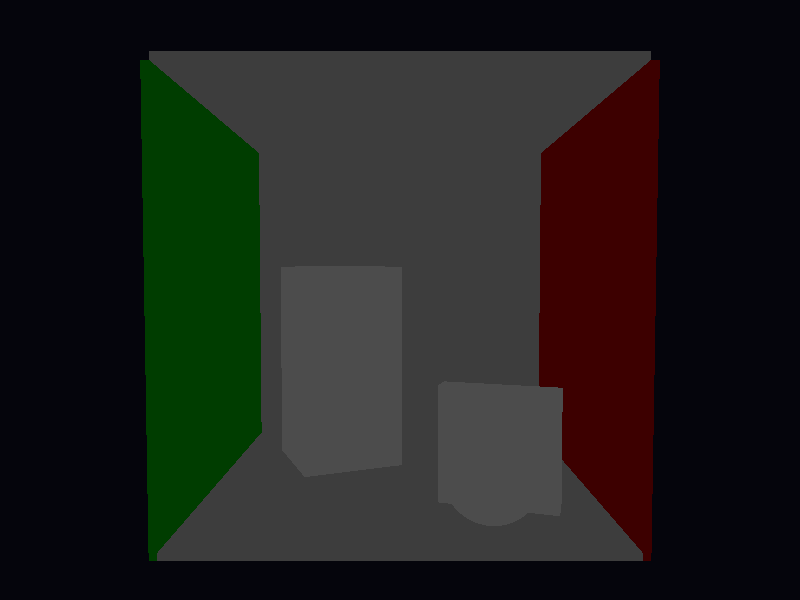
\includegraphics[width=0.98\linewidth]{../outputs/proj1_req1_geometry_20260502_121509/render.png}
\caption{Cena de geometria e instanciação: dois \texttt{Instance(Box)} e uma \texttt{Sphere} sob câmera fixa e iluminação ambiente (800x600, spp=1).}
\label{fig:req1-v3}
\figcmd{python -m ray_tracing_2.proj1_req1_geometry --width 800 --height 600 --sampling_mode center --spp 1}
\end{figure}

\subsection{Iluminação local com múltiplas fontes pontuais}
\label{sec:fig-luzes-v3}

Na Figura~\ref{fig:req2-v3}, a presença de três \texttt{PointLight} torna visível a contribuição angular de fontes distintas sobre materiais diferentes. O efeito importante da cena é pedagógico: ela torna fácil perceber que a componente especular não depende apenas da posição da luz, mas também do material e do ponto de vista. As duas esferas com \texttt{shininess} diferente cumprem exatamente esse papel.

\begin{figure}[!ht]
\centering
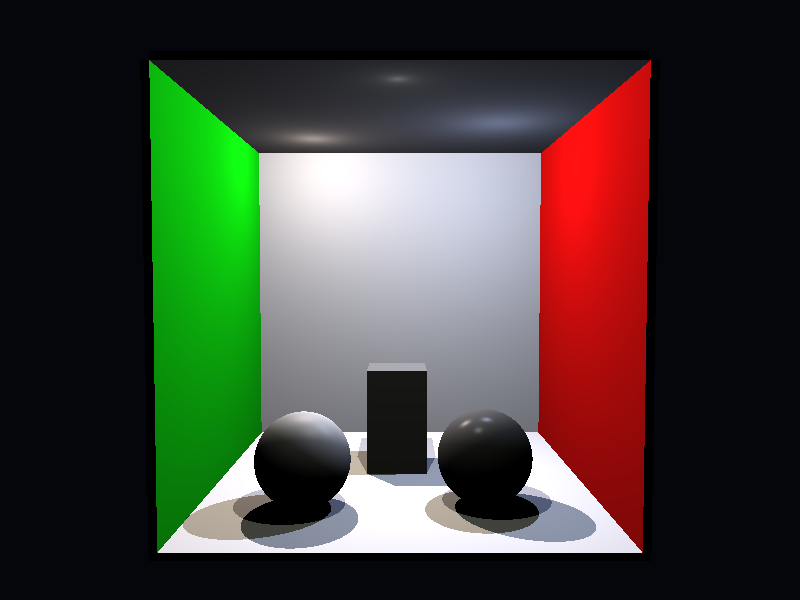
\includegraphics[width=0.98\linewidth]{../outputs/proj1_req2_point_lights_20260502_121731/render.png}
\caption{Cena com múltiplas luzes pontuais e variação do brilho especular em materiais com \texttt{shininess} distinto no baseline \texttt{center} (800x600, spp=1, tempo de render aproximado de 19,66\,s).}
\label{fig:req2-v3}
\figcmd{python -m ray_tracing_2.proj1_req2_point_lights --width 800 --height 600 --sampling_mode center --spp 1}
\end{figure}

Como exemplo simples de comparação de antialiasing sobre a mesma configuração geométrica e fotométrica, a Figura~\ref{fig:req2-aa-v3} repete essa cena com \texttt{stratified} e \(25\) amostras por pixel. A diferença visual não altera a leitura física da cena, mas reduz serrilhados e estabiliza bordas e \emph{highlights} especulares ao custo de um crescimento expressivo no número total de raios.

\begin{figure}[!ht]
\centering
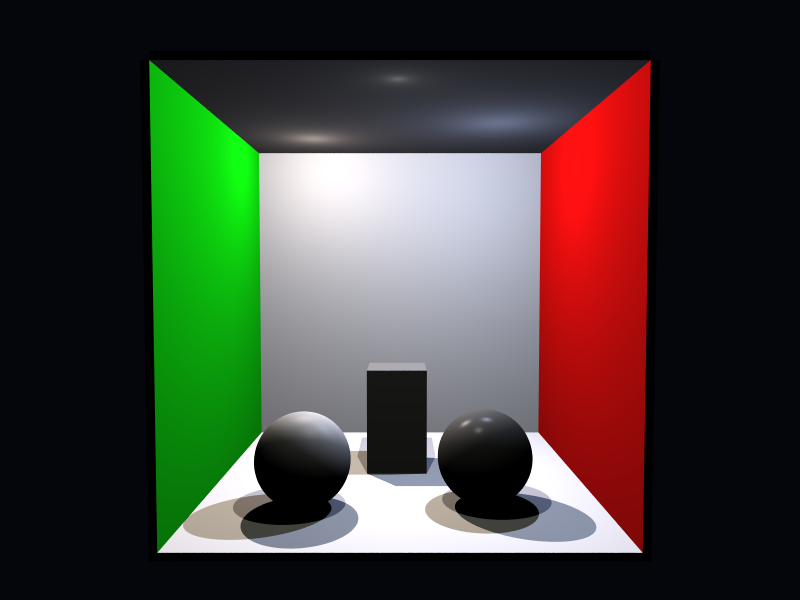
\includegraphics[width=0.98\linewidth]{../outputs/proj1_req2_point_lights_20260502_192411/render.png}
\caption{Mesma cena de múltiplas luzes pontuais com \texttt{sampling\_mode=stratified} e \(25\) amostras por pixel: melhora a integração espacial sem alterar materiais, luzes ou câmera (800x600, tempo de render aproximado de 501,91\,s).}
\label{fig:req2-aa-v3}
\figcmd{python -m ray_tracing_2.proj1_req2_point_lights --width 800 --height 600 --sampling_mode stratified --spp 25 --seed 42}
\end{figure}

\subsection{Phong e sombras diretas}
\label{sec:fig-phong-v3}

Esta cena foi escolhida para expor o núcleo fotométrico mínimo do projeto. Na Figura~\ref{fig:req3-v3}, a leitura correta é que o mesmo pipeline decide qual superfície foi atingida e, depois, se cada luz contribui ou não para aquele ponto. O contraste entre o vermelho mais fosco e o azul mais brilhante ajuda a separar visualmente o termo difuso da concentração angular do termo especular.

\begin{figure}[!ht]
\centering
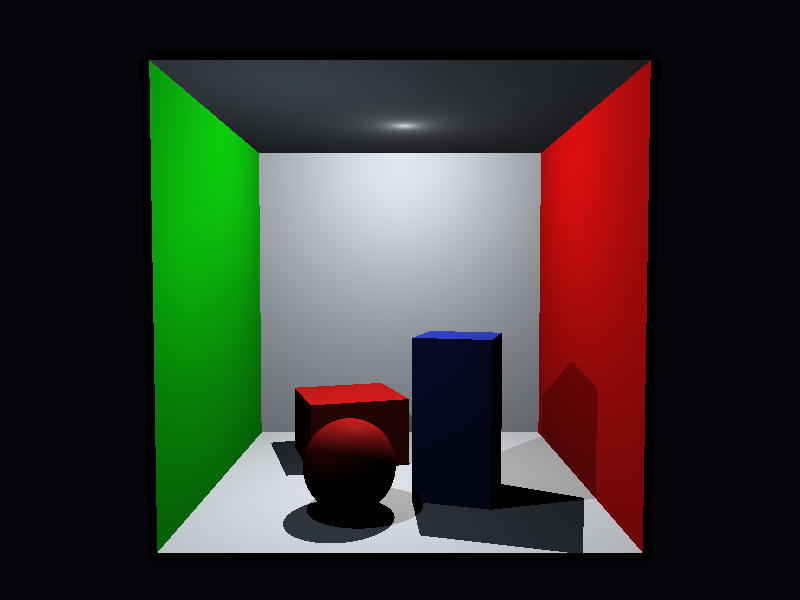
\includegraphics[width=0.98\linewidth]{../outputs/proj1_req3_phong_shadows_20260502_121809/render.png}
\caption{Cena de sombreamento local com Phong e sombras diretas duras por visibilidade até a fonte (800x600, spp=1).}
\label{fig:req3-v3}
\figcmd{python -m ray_tracing_2.proj1_req3_phong_shadows --width 800 --height 600 --sampling_mode center --spp 1}
\end{figure}

\subsection{Amostragem sobre o pixel}
\label{sec:fig-aa-v3}

Na Figura~\ref{fig:req4-v3}, a geometria foi escolhida para que arestas finas e contrastes fortes deixem o aliasing visível. As três imagens seguintes usam a mesma câmera, a mesma geometria, as mesmas luzes e o mesmo enquadramento; o que muda é apenas a estratégia de amostragem do pixel. O ponto importante não é provar convergência estatística, mas deixar claro que a base já separa câmera, geometria e amostragem do pixel, o que permite comparar regimes de integração sem reconfigurar o restante da cena.

\begin{figure}[!ht]
\centering
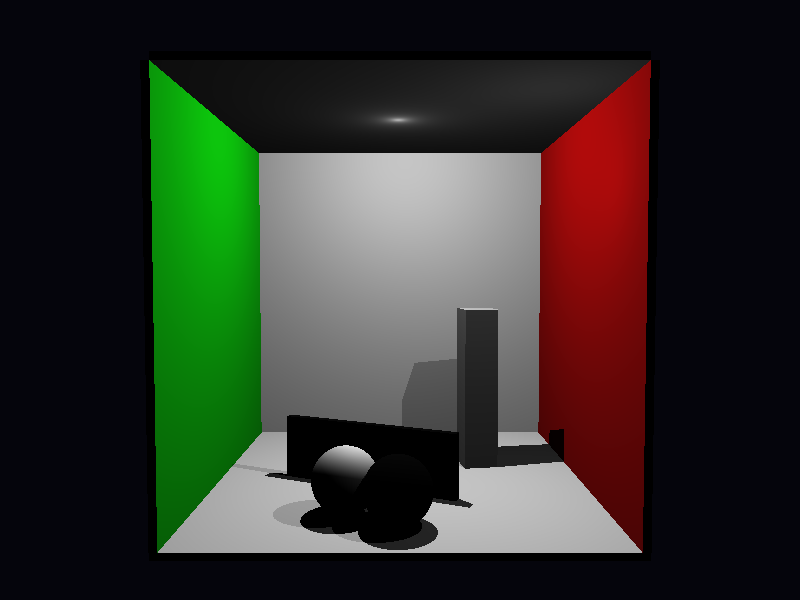
\includegraphics[width=0.98\linewidth]{../outputs/proj1_req4_sampling_20260502_122009/render.png}
\caption{Cena-base para comparação entre \texttt{center}, \texttt{jittered} e \texttt{stratified} no domínio do pixel (800x600, \texttt{sampling\_mode=center}, spp=1, tempo de render aproximado de 20,65\,s).}
\label{fig:req4-v3}
\figcmd{python -m ray_tracing_2.proj1_req4_sampling --width 800 --height 600 --sampling_mode center --spp 1}
\end{figure}

\begin{figure}[!ht]
\centering
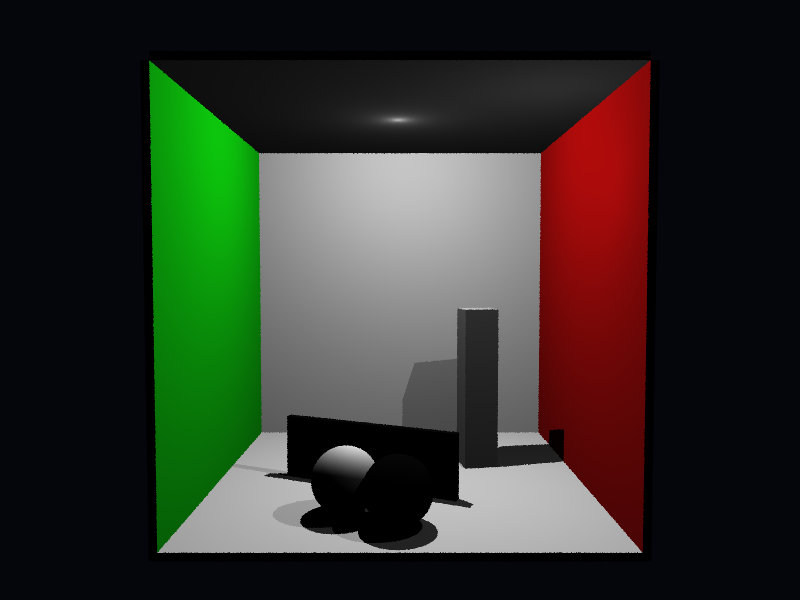
\includegraphics[width=0.98\linewidth]{../outputs/proj1_req4_sampling_20260506_211723/render.png}
\caption{Mesma cena de antialiasing com \texttt{sampling\_mode=jittered} e \(4\) amostras por pixel: o serrilhado estruturado vira ruído espacial mais difuso, com tempo de render aproximado de 86,56\,s.}
\label{fig:req4-jittered-v3}
\figcmd{python -m ray_tracing_2.proj1_req4_sampling --width 800 --height 600 --sampling_mode jittered --spp 4 --seed 42}
\end{figure}

\begin{figure}[!ht]
\centering
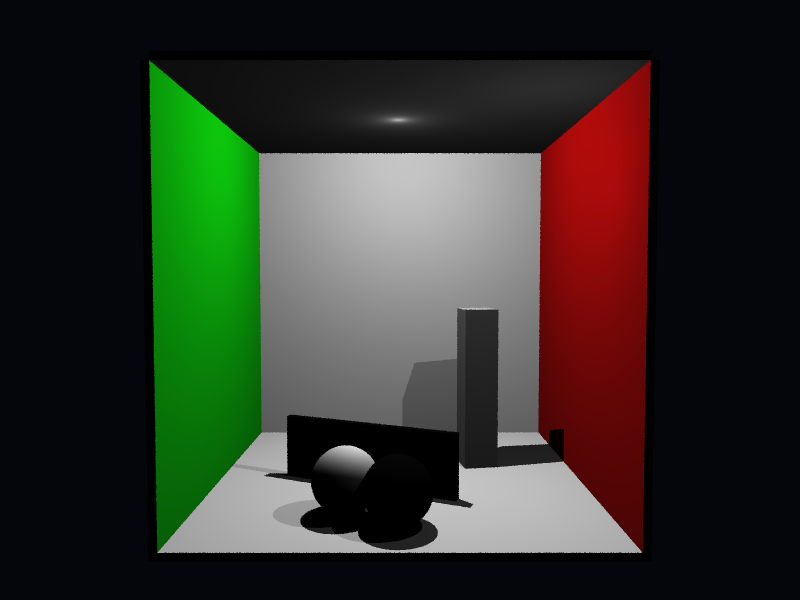
\includegraphics[width=0.98\linewidth]{../outputs/proj1_req4_sampling_20260506_211923/render.png}
\caption{Mesma cena de antialiasing com \texttt{sampling\_mode=stratified} e \(4\) amostras por pixel: a cobertura espacial mais uniforme do pixel reduz ruído e estabiliza contornos em relação ao \texttt{jittered}, com tempo de render aproximado de 84,84\,s.}
\label{fig:req4-stratified-v3}
\figcmd{python -m ray_tracing_2.proj1_req4_sampling --width 800 --height 600 --sampling_mode stratified --spp 4 --seed 42}
\end{figure}

Lidas em sequência, as Figuras~\ref{fig:req4-v3}, \ref{fig:req4-jittered-v3} e \ref{fig:req4-stratified-v3} mostram exatamente o ganho pedagógico do requisito de amostragem múltipla: \texttt{center} preserva o baseline determinístico e barato; \texttt{jittered} quebra o padrão regular do aliasing ao espalhá-lo como ruído; e \texttt{stratified} cobre o pixel de forma mais uniforme, mantendo custo muito próximo ao do \texttt{jittered}, mas com leitura visual mais estável.

\subsection{Malha triangular com BVH local}
\label{sec:fig-bvh-v3}

A Figura~\ref{fig:rext-bvh-v3} sintetiza a parte mais importante do bloco de triângulos e aceleração. A evidência principal não é apenas que a malha aparece na imagem, mas que ela participa do mesmo pipeline de materiais e luzes e, ao mesmo tempo, é percorrida por uma BVH local. Essa figura deve ser lida em conjunto com a discussão teórica da seção anterior: o ganho é real para a malha, mas não autoriza falar em acelerador global da cena.

\begin{figure}[!ht]
\centering
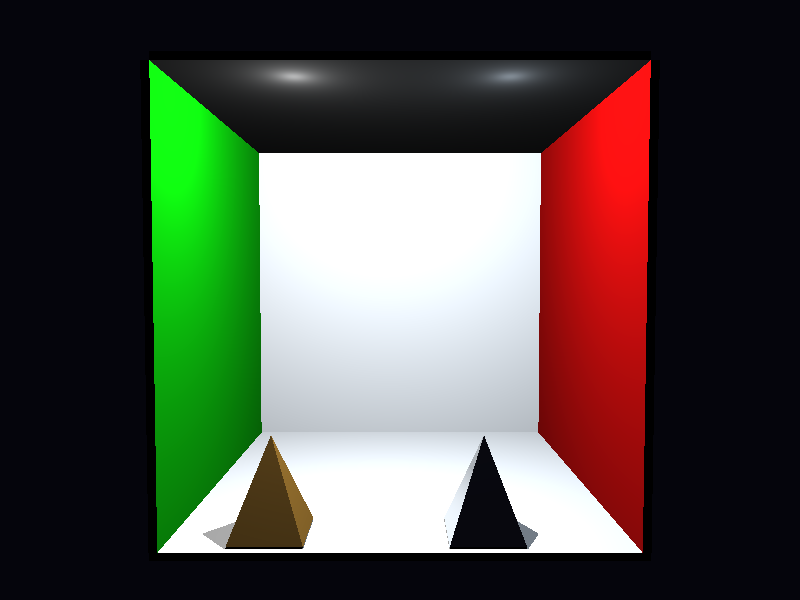
\includegraphics[width=0.98\linewidth]{../outputs/proj1_rext_bvh_20260502_131902/render.png}
\caption{Cena triangular com BVH local: a imagem visualiza a malha sob o mesmo pipeline de iluminação, enquanto a poda por AABB reduz o custo interno da interseção (800x600, spp=1).}
\label{fig:rext-bvh-v3}
\figcmd{python -m ray_tracing_2.proj1_rext_bvh --width 800 --height 600 --sampling_mode center --spp 1}
\end{figure}

\subsection{Luz de área e emissor visível}
\label{sec:fig-area-v3}

Na Figura~\ref{fig:rext-area-light-v3}, a leitura relevante é dupla. Primeiro, a cena mostra que a luz de área produz penumbra por amostragem espacial do emissor. Segundo, ela registra uma decisão de arquitetura que a parte teórica precisa explicar: a luminária visível é obtida por \texttt{EmissiveMaterial}, enquanto a iluminação direta da cena continua a vir da \texttt{AreaLight}. Em outras palavras, o painel aceso visto pela câmera e a fonte utilizada para \emph{shadow rays} não são a mesma camada de abstração.

\begin{figure}[!ht]
\centering
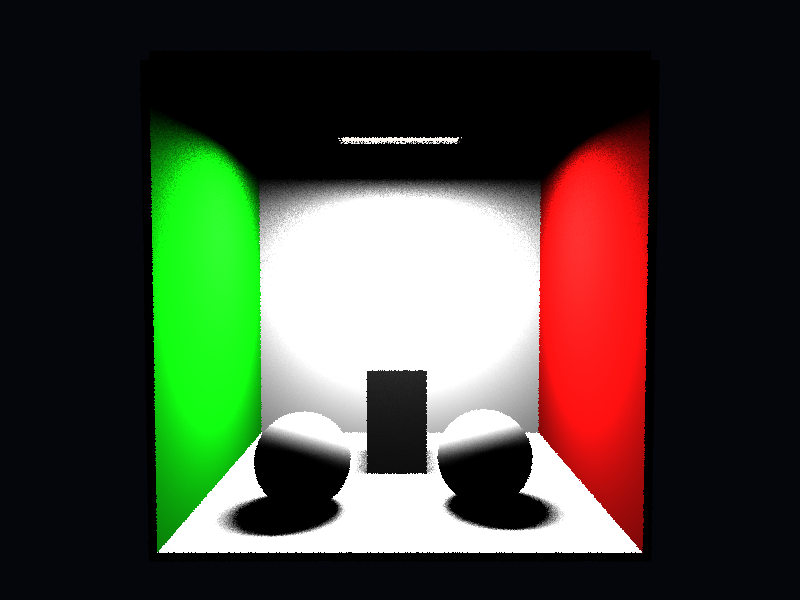
\includegraphics[width=0.98\linewidth]{../outputs/proj1_rext_area_light_20260502_150206/render.png}
\caption{Cena com luz de área retangular e emissor visível: a penumbra vem da fonte extensa amostrada, enquanto a aparência luminosa do painel vem de \texttt{EmissiveMaterial} (800x600, spp=1).}
\label{fig:rext-area-light-v3}
\figcmd{python -m ray_tracing_2.proj1_rext_area_light --width 800 --height 600 --sampling_mode center --spp 1}
\end{figure}

\subsection{Refração, TIR e Beer-Lambert}
\label{sec:fig-refracao-v3}

A Figura~\ref{fig:rext-refractive-v3} concentra a parte óptica mais avançada da base. A cena não prova isoladamente cada equação, mas é a melhor evidência integrada de que direção refratada, reflexão interna total e atenuação no interior do meio passaram a participar do mesmo fluxo de visibilidade e recursão. O ponto metodológico importante é este: o resultado visual não aparece como módulo separado, e sim como extensão do mesmo traçador que já tratava Phong e sombras diretas.

\begin{figure}[!ht]
\centering
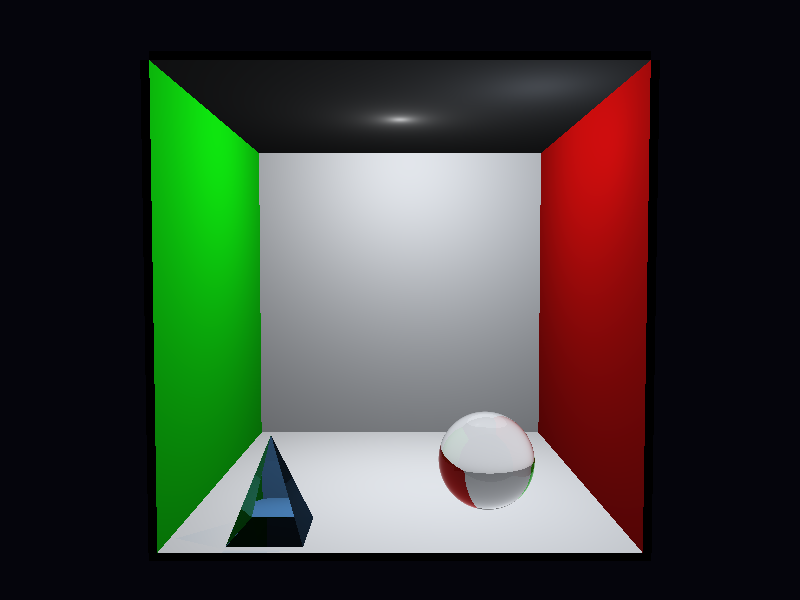
\includegraphics[width=0.98\linewidth]{../outputs/proj1_rext_refractive_20260502_132340/render.png}
\caption{Cena com material refratário: o resultado combina Lei de Snell, reflexão interna total e atenuação tipo Beer-Lambert dentro do mesmo pipeline recursivo (800x600, spp=1).}
\label{fig:rext-refractive-v3}
\figcmd{python -m ray_tracing_2.proj1_rext_refractive --width 800 --height 600 --sampling_mode center --spp 1}
\end{figure}

\subsection{AA em uma cena integrada}
\label{sec:fig-cornell-aa-v3}

Uma segunda comparação, agora em uma cena mais rica, serve para verificar se a leitura feita em \texttt{req4} persiste quando a imagem concentra mais oclusões e contraste local. As Figuras~\ref{fig:cornell-center-v3} e \ref{fig:cornell-stratified-v3} usam a mesma \emph{Cornell box} com pirâmide interna; o ganho do \texttt{stratified} continua qualitativo, mas aparece agora sob custo bem mais alto, o que ajuda a separar melhoria visual de viabilidade computacional.

\begin{figure}[!ht]
\centering
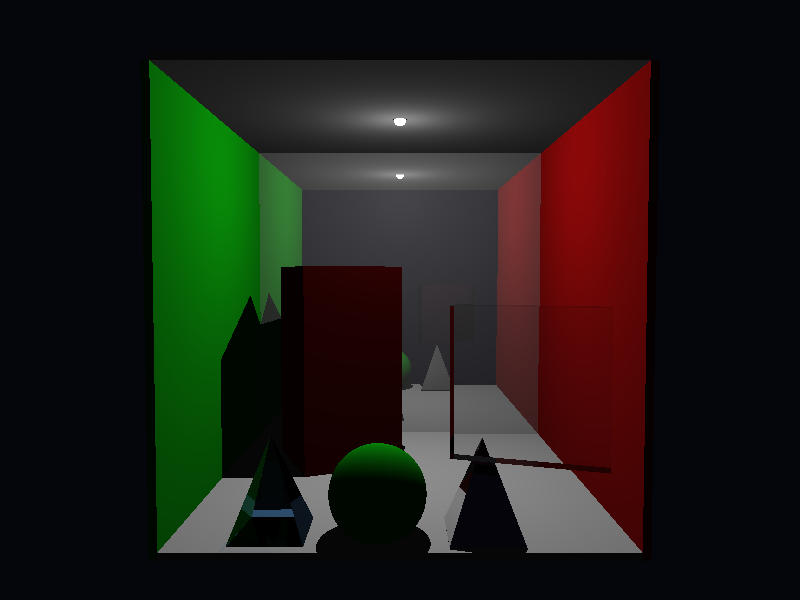
\includegraphics[width=0.98\linewidth]{../outputs/cornell_box_pyramid_20260502_190902/render.png}
\caption{Cena integrada \emph{Cornell box} com pirâmide no baseline \texttt{center}: referência para avaliar como aliasing e ruído aparecem em uma composição mais rica (800x600, spp=1, tempo aproximado de 49,76\,s).}
\label{fig:cornell-center-v3}
\figcmd{python -m ray_tracing_2.cornell_box_pyramid --width 800 --height 600 --sampling_mode center --spp 1}
\end{figure}

\begin{figure}[!ht]
\centering
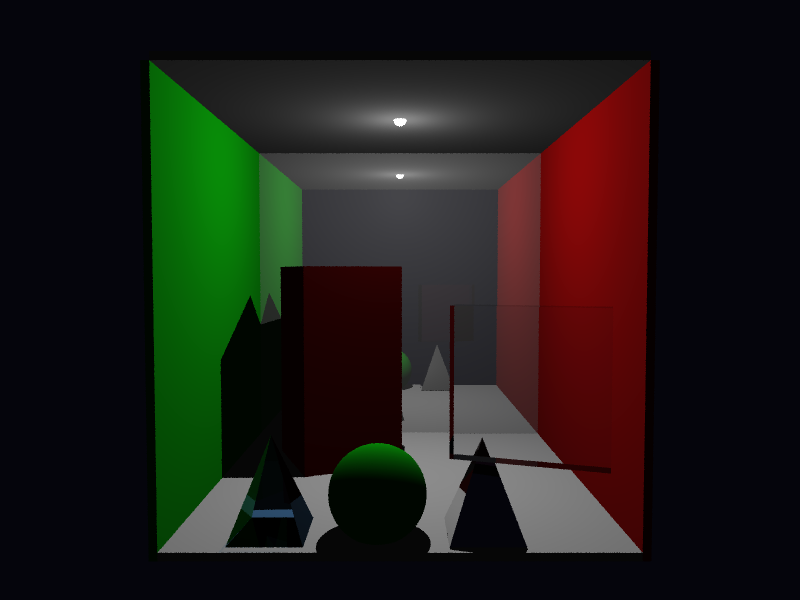
\includegraphics[width=0.98\linewidth]{../outputs/cornell_box_pyramid_20260502_191034/render.png}
\caption{Mesma cena integrada com \texttt{sampling\_mode=stratified} e \(4\) amostras por pixel: a melhoria observada em \texttt{req4} reaparece em uma imagem mais carregada, ao custo de aproximadamente 200,80\,s.}
\label{fig:cornell-stratified-v3}
\figcmd{python -m ray_tracing_2.cornell_box_pyramid --width 800 --height 600 --sampling_mode stratified --spp 4 --seed 42}
\end{figure}

\subsection{Cenas integradas recuperadas por snapshots}
\label{sec:fig-recuperadas-v3}

Os exemplos anexados de cenas finais merecem aparecer também como evidência visual, e não apenas como números citados na subseção de infraestrutura experimental. As Figuras~\ref{fig:proj1-final-v3}, \ref{fig:proj1-final-v2} e \ref{fig:heart-triangle-v3} mostram três casos em que a imagem permanece legível justamente porque o snapshot preserva o contexto técnico necessário para interpretá-la. Nas duas cenas finais, a câmera e o regime básico de render permanecem estáveis, o que torna comparável a diferença entre \(144{,}2\,s\) e \(172{,}0\,s\); na cena da malha cardíaca, o registro de \texttt{spp=25} e acelerador \texttt{bvh} impede que o alto custo apareça como dado solto.

\begin{figure}[!ht]
\centering
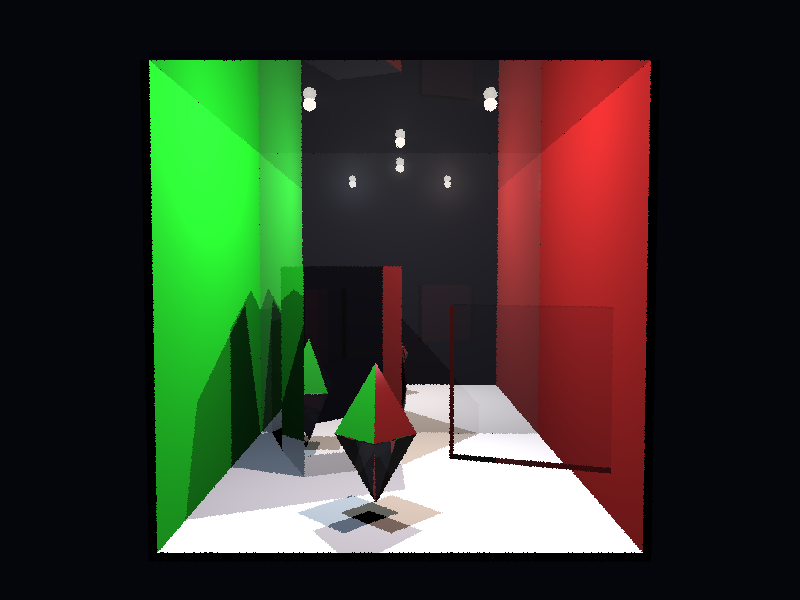
\includegraphics[width=0.98\linewidth]{../outputs/proj1_final_20260502_201946/render.png}
\caption{Cena final integrada \texttt{proj1\_final}: combinação de materiais reflexivos, refratários e malhas triangulares em um caso no qual o estimador prevê \(63{,}6\,s\), mas o render observado chega a \(144{,}2\,s\).}
\label{fig:proj1-final-v3}
\figcmd{python -m ray_tracing_2.proj1_final --width 800 --height 600 --spp 1}
\end{figure}

\begin{figure}[!ht]
\centering
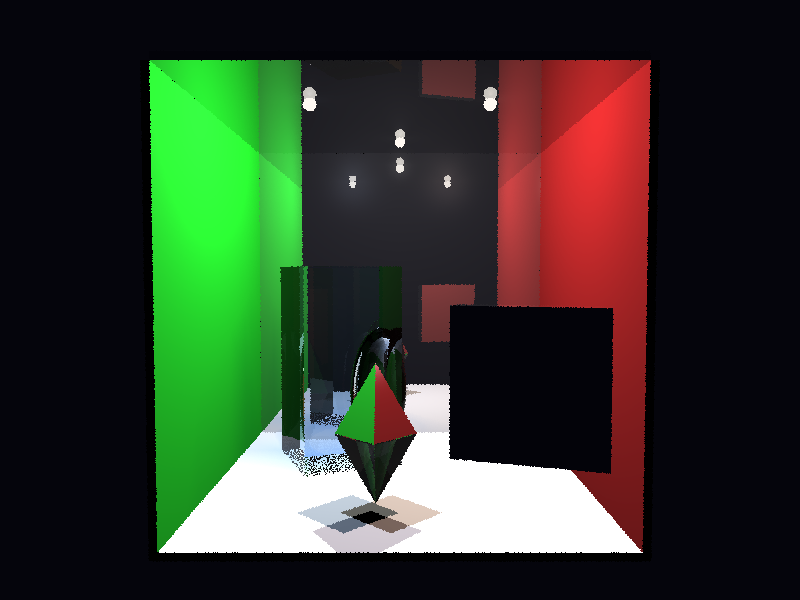
\includegraphics[width=0.98\linewidth]{../outputs/proj1_final_v2_20260502_202707/render.png}
\caption{Variante \texttt{proj1\_final\_v2}: mesma leitura de cena integrada sob câmera equivalente, agora com tempo real de \(172{,}0\,s\) para uma previsão de \(74{,}3\,s\), reforçando a sensibilidade do custo à composição geométrica e material.}
\label{fig:proj1-final-v2}
\figcmd{python -m ray_tracing_2.proj1_final_v2 --width 800 --height 600 --spp 1}
\end{figure}

\begin{figure}[!ht]
\centering
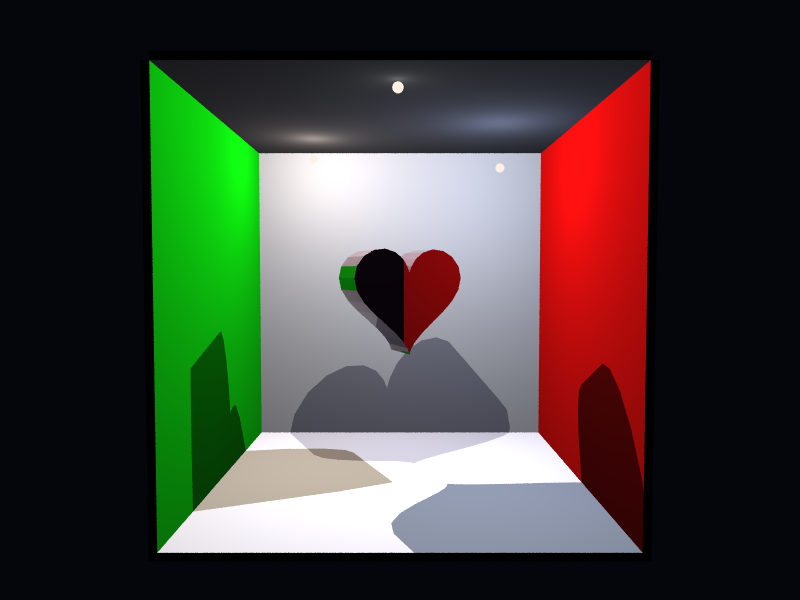
\includegraphics[width=0.98\linewidth]{../outputs/proj1_heart_trianglemesh_20260502_205136/render.png}
\caption{Cena \texttt{proj1\_heart\_trianglemesh}: malha triangulada com \texttt{bvh} e \(25\) amostras por pixel, em um caso onde a estimativa \(1122{,}4\,s\) permanece relativamente próxima do tempo observado \(1008{,}0\,s\).}
\label{fig:heart-triangle-v3}
\figcmd{python -m ray_tracing_2.proj1_heart_trianglemesh --width 800 --height 600 --spp 25 --sampling_mode jittered}
\end{figure}

Os demais artefatos exploratórios recuperados via snapshot -- da cena mínima \texttt{main\_scene} a variações sucessivas de \texttt{cornell\_box} e a uma versão adicional de \texttt{cornell\_box\_pyramid} -- ficam reunidos no Anexo C. Eles não são centrais para a progressão teórica do corpo principal, mas ajudam a mostrar que a instrumentação do projeto preservou evidência útil também fora do conjunto canônico de cenas escolhido para a narrativa principal.

\section{Decisões de Modelagem e Limites}
\label{sec:limites-v3}

\subsection{Convenções radiométricas}
\label{sec:lim-radiometria-v3}

O projeto não usa a mesma convenção radiométrica para todas as fontes. \texttt{PointLight} preserva a interpretação simplificada do enunciado e trata \texttt{power} como radiância incidente constante, sem fator explícito de decaimento por \(1/r^2\). Já \texttt{AreaLight} distribui energia pelas amostras do emissor e introduz atenuação geométrica com a distância, além de um termo angular de emissão. Essa heterogeneidade é aceitável no contexto didático do Projeto 1, mas precisa ser declarada para evitar leitura física mais forte do que a base sustenta: cenas que misturam essas duas fontes são visualmente úteis, porém não definem uma convenção radiométrica unificada.

\subsection{Câmera e formação de imagem}
\label{sec:lim-camera-v3}

Toda a formação de imagem permanece no modelo pinhole~\slidescite{inf2608slides04}{19--39}. Isso significa que \texttt{focal\_distance} controla apenas a geometria do plano de projeção. Não há lente fina, abertura finita nem profundidade de campo. O supersampling melhora a integração sobre o pixel, mas não muda a física da câmera. Portanto, as imagens devem ser lidas como resultados de câmera pinhole com amostragem estocástica, e não como simulações ópticas completas.

\subsection{Aceleração e complexidade de cena}
\label{sec:lim-aceleracao-v3}

A parte de triângulos e aceleração cobre apenas uma fração do arco teórico da disciplina. Há BVH estática por \texttt{TriangleMesh}, com AABB e travessia recursiva simplificada, mas não há grade regular, SAH\footnote{\emph{Surface Area Heuristic}, heurística clássica para particionamento de BVHs que não é implementada nesta base.}, BVH linearizada nem estrutura global de aceleração. Em termos de custo, isso significa que a interseção no topo da cena continua linear no número de objetos, e o ganho de desempenho aparece apenas dentro das malhas trianguladas.

\subsection{Materiais recursivos e truncamento}
\label{sec:lim-recursao-v3}

Os materiais reflexivos e refratários ampliam bastante o escopo do projeto, mas continuam sendo aproximações controladas. A recursão é truncada por \texttt{max\_depth}, o que contém o custo computacional e evita crescimento explosivo do número de raios, ao preço de interromper cadeias longas de reflexão e transmissão. Além disso, a combinação entre Phong local, Fresnel-Schlick, Snell, TIR e Beer-Lambert deve ser lida como composição fenomenológica: ela preserva efeitos ópticos relevantes para o escopo didático, mas não fecha balanço energético rigoroso nem substitui um modelo completo de transporte global de luz. No caso da refração, a própria Beer-Lambert é aplicada como aproximação homogênea e a detecção de TIR ainda passa por um critério heurístico na implementação.

\section{Conclusão}
\label{sec:conclusao-v3}

Tomando o estado atual do repositório como objeto de análise, o projeto reúne um núcleo geométrico e fotométrico coerente: raio paramétrico, interseções analíticas, câmera pinhole, filme com suporte a supersampling, sombreamento local de Phong e sombras diretas. Sobre esse núcleo, a base acrescenta extensões relevantes do conteúdo da disciplina, como instanciação afim, luz de área, reflexão especular com Fresnel-Schlick, refração dielétrica com Lei de Snell, Beer-Lambert e uma BVH local para malhas triangulares. O mérito técnico central está justamente nessa continuidade: as extensões não substituem o pipeline inicial, mas o tensionam sem romper sua lógica de composição entre câmera, interseção, material e visibilidade.

O relatório também mostra que essa coerência arquitetural não equivale a completude física. A câmera permanece estritamente pinhole; as fontes de luz não compartilham uma convenção radiométrica única; a ótica recursiva combina Phong, Schlick, Snell e Beer-Lambert como aproximações controladas; e a aceleração permanece local às malhas trianguladas, sem estrutura global de cena. Em outras palavras, a base é tecnicamente consistente como implementação didática e como ponto de partida para extensões mais ambiciosas, mas não se propõe, neste estágio, a um renderer fisicamente completo. Esse ponto merece destaque porque organiza corretamente o valor do trabalho e, ao mesmo tempo, indica uma direção clara de aprofundamento: avançar além daqui passa por consolidar o domínio de álgebra linear, óptica geométrica e métodos numéricos exigido por modelagens mais rigorosas.

É justamente por isso que os limites identificados apontam mais para fronteiras de arquitetura do que para falhas do núcleo atual. Tornar a base radiometricamente uniforme, substituir heurísticas ópticas por testes mais rigorosos, incorporar integração volumétrica mais completa ou acelerar a cena inteira com uma estrutura global exigiria revisão de abstrações, e não apenas adição local de mais um recurso. Avaliado nesse enquadramento, o repositório entrega um ray tracer educacional reprodutível, tecnicamente defensável e bem localizado dentro do arco da disciplina: não pretende cobrir integralmente o problema de síntese física de imagens, mas já oferece uma implementação consistente de uma parcela substantiva desse problema e uma base clara para aprofundamento teórico e experimental.

\bibliographystyle{apalike-sol}
\bibliography{refs}

\clearpage
\section*{Anexo A: Quadros Consolidados de Referência e Evidência}

Os quadros a seguir sintetizam a ligação entre os conceitos de referência discutidos no corpo do texto e a evidência mais direta encontrada na base. A coluna \emph{Nota} registra, em forma compacta, as páginas dos slides, as referências externas mais próximas e as linhas de código mais relevantes para cada conceito.

\subsection*{Núcleo geométrico e fotométrico}

\begin{table*}[!ht]
\caption{Quadro consolidado do núcleo geométrico e fotométrico.}
\centering
\begin{tblr}{
width=\textwidth,
colspec={Q[l,wd=0.25\textwidth] Q[l,wd=0.33\textwidth] Q[l,wd=0.34\textwidth]},
row{1}={font=\bfseries},
rows={valign=t},
cells={font=\small}
}
Conceito de referência & Evidência principal & Nota \\
Raio paramétrico, visibilidade e registro de hit & \texttt{Ray}, \texttt{Hit}, \texttt{Scene.compute\_intersection()}, \texttt{Scene.trace\_ray()} & Slides 04, pp.~7--9; \pbrtsecpair{1.2}{3.5}; \texttt{hit.py:11, 25}; \texttt{scene.py:33, 137}. \\
Interseções raio-plano e raio-esfera & \texttt{Sphere.intersect()}, \texttt{Plane.intersect()}, deslocamento por \(\varepsilon\) em \texttt{offset\_point()} & Slides 04, pp.~10--18; \texttt{shape.py:17, 23, 54, 60}; \texttt{scene.py:50}. \\
Câmera pinhole, filme e geração de raios primários & \texttt{Camera.generate\_ray()}, \texttt{Film.get\_sample()}, \texttt{Film.get\_samples\_for\_pixel()}, \texttt{Film.render()} & Slides 04, pp.~19--39; \pbrtsec{5.2}; \texttt{camera.py:6, 28}; \texttt{film.py:74, 98, 104, 156}. \\
Modelo local de Phong, ambiente e sombras diretas & \texttt{PhongMaterial.direct\_lighting()}, \texttt{PhongMaterial.eval()}, \texttt{PointLight.radiance()}, \texttt{Scene.transmittance()} & Slides 04, pp.~40--55; \texttt{material.py:70, 79, 106}; \texttt{light.py:51, 55}; \texttt{scene.py:66}. \\
Convenção simplificada para fonte pontual & \texttt{PointLight.radiance()} sem fator explícito de \(1/r^2\) & Slides 04, pp.~40--55; escolha didática coerente com o enunciado; \texttt{light.py:51, 55}. \\
Pipeline câmera--interseção--material & \texttt{Film.render()}, \texttt{Camera.generate\_ray()}, \texttt{Scene.compute\_intersection()}, \texttt{Scene.trace\_ray()} & Slides 04, pp.~44--55; \texttt{film.py:156}; \texttt{camera.py:28}; \texttt{scene.py:33, 137}. \\
\end{tblr}
\end{table*}

\subsection*{Extensões ópticas, amostrais e de transformação}

\begin{table*}[!ht]
\caption{Quadro consolidado das extensões ópticas, amostrais e de transformação.}
\centering
\begin{tblr}{
width=\textwidth,
colspec={Q[l,wd=0.25\textwidth] Q[l,wd=0.33\textwidth] Q[l,wd=0.34\textwidth]},
row{1}={font=\bfseries},
rows={valign=t},
cells={font=\small}
}
Conceito de referência & Evidência principal & Nota \\
Antialiasing por múltiplas amostras no pixel & \texttt{uniform\_samples\_2d()}, \texttt{stratified\_grid\_samples\_2d()}, \texttt{Film.get\_samples\_for\_pixel()} & Slides 05, pp.~4--8; \pbrtsecpair{8.1}{8.5}; \texttt{sampling.py:15, 27, 43}; \texttt{film.py:104, 156}. \\
Instanciação afim e transformação correta de normais & \texttt{Instance.intersect()} com uso de inversa e inversa transposta & Slides 05, pp.~9--13; \pbrtsec{3.5}; \texttt{shape.py:253, 262}. \\
Luz de área, amostragem do emissor, penumbra e emissor visível & \texttt{AreaLight.sample\_radiance()}, \texttt{AreaLight.radiance()}, \texttt{EmissiveMaterial.eval()} & Slides 05, pp.~14--23; \pbrtsec{12.4}; \texttt{light.py:80, 135, 195}; \texttt{material.py:37, 50}. \\
Caixa, AABB e método de slabs & \texttt{Box.intersect()}, \texttt{AABB.intersects()} & Slides 05, pp.~24--25; \pbrtsec{3.7}; \texttt{shape.py:74, 88}; \texttt{triangle\_bvh.py:50, 65}. \\
Traçador recursivo com profundidade finita & \texttt{Scene.can\_spawn\_ray()}, \texttt{Scene.trace\_ray()} & Slides 05, pp.~26--35; \texttt{scene.py:59, 137}. \\
Reflexão especular com Fresnel-Schlick & \texttt{ReflectiveMaterial.eval()} & Slides 05, pp.~26--28; \pbrtsec{9.3}; \texttt{material.py:118, 136}. \\
Refração dielétrica, TIR e Beer-Lambert & \texttt{TransparentMaterial.eval()}, \texttt{shadow\_transmittance()} & Slides 05, pp.~29--35; \pbrtsecpair{9.5}{11.2}; \texttt{material.py:176, 206, 227}. \\
Transmitância acumulada em raios de sombra & \texttt{Scene.transmittance()} e delegação para \texttt{shadow\_transmittance()} & Slides 05, pp.~33--35; \texttt{scene.py:66}; \texttt{material.py:30, 61, 206}. \\
\end{tblr}
\end{table*}

\subsection*{Infraestrutura experimental e reprodutibilidade}

\begin{table*}[!ht]
\caption{Quadro consolidado da infraestrutura experimental e da reprodutibilidade.}
\centering
\begin{tblr}{
width=\textwidth,
colspec={Q[l,wd=0.25\textwidth] Q[l,wd=0.33\textwidth] Q[l,wd=0.34\textwidth]},
row{1}={font=\bfseries},
rows={valign=t},
cells={font=\small}
}
Conceito de referência & Evidência principal & Nota \\
CLI padronizada para execuções comparáveis & \texttt{CommonRenderOptions} e conversão uniforme de parâmetros para \emph{entrypoints} e estimador & Camada de engenharia que estabiliza resolução, \texttt{spp}, \texttt{sampling\_mode}, semente e calibração; \texttt{cli.py:16, 50, 64, 96, 174}. \\
Snapshot persistente do estado do render & \texttt{RenderSnapshot.from\_runtime()} e serialização em \texttt{properties.json}/\texttt{properties.md} & Registra render, câmera, cena, objetos e luzes em artefatos auditáveis; \texttt{render\_snapshot.py:524, 605, 656, 665, 770, 773}. \\
Estimativa, calibração e comparação com o tempo real & \texttt{RayCountEstimator} e execução coordenada por \texttt{RenderEstimator} & Mede throughput, atualiza o modelo e persiste o comparativo estimado/real ao fim do render; \texttt{render\_estimator.py:34, 189, 277, 368, 389, 492}. \\
\end{tblr}
\end{table*}

\subsection*{Geometria triangular e aceleração local}

\begin{table*}[!ht]
\caption{Quadro consolidado da geometria triangular e da aceleração local.}
\centering
\begin{tblr}{
width=\textwidth,
colspec={Q[l,wd=0.25\textwidth] Q[l,wd=0.33\textwidth] Q[l,wd=0.34\textwidth]},
row{1}={font=\bfseries},
rows={valign=t},
cells={font=\small}
}
Conceito de referência & Evidência principal & Nota \\
Triângulo como primitiva elementar e normal orientada & \texttt{Triangle}, vetores de aresta \texttt{e1}/\texttt{e2}, normal geométrica & Slides 06, pp.~3--4; \texttt{shape.py:144}. \\
Interseção raio-triângulo por Möller--Trumbore & \texttt{Triangle.intersect()} & Slides 06, pp.~5--12; \texttt{shape.py:158}. \\
Malha triangulada integrada ao pipeline geral & \texttt{TriangleMesh}, \texttt{TriangleMesh.intersect()}, \texttt{Scene.compute\_intersection()} & Slides 06, pp.~13--14; \texttt{shape.py:188, 241}; \texttt{scene.py:33}. \\
BVH local para malhas trianguladas & \texttt{TriangleBVH}, \texttt{TriangleBVHNode.intersect()}, \texttt{TriangleBVH.\_build()} & Slides 06, pp.~22--36; \pbrtsec{7.3}; \texttt{triangle\_bvh.py:104, 115, 146, 160, 198}. \\
AABB como volume de contenção & \texttt{AABB}, \texttt{AABB.intersects()} & Slides 06, pp.~22--36; \texttt{triangle\_bvh.py:50, 65}. \\
Percurso sequencial no topo da cena & \texttt{Scene.compute\_intersection()} como evidência da ausência de agregador global & Slides 06, pp.~22--36; \texttt{scene.py:33}. \\
\end{tblr}
\end{table*}

\clearpage
\section*{Anexo B: Diagramas de Classes}

Este anexo passa a reunir duas leituras complementares da arquitetura principal do pacote \texttt{ray\_tracing\_2}. A primeira preserva a versão inicial do diagrama, mais compacta e centrada no pipeline geométrico e fotométrico. A segunda, \texttt{v3}, estende essa base para incluir a camada de CLI, estimativa/calibração e snapshots, que hoje participa diretamente da reprodutibilidade experimental discutida no corpo do texto.

\subsection*{Versão inicial}

\begin{figure*}[!ht]
\centering
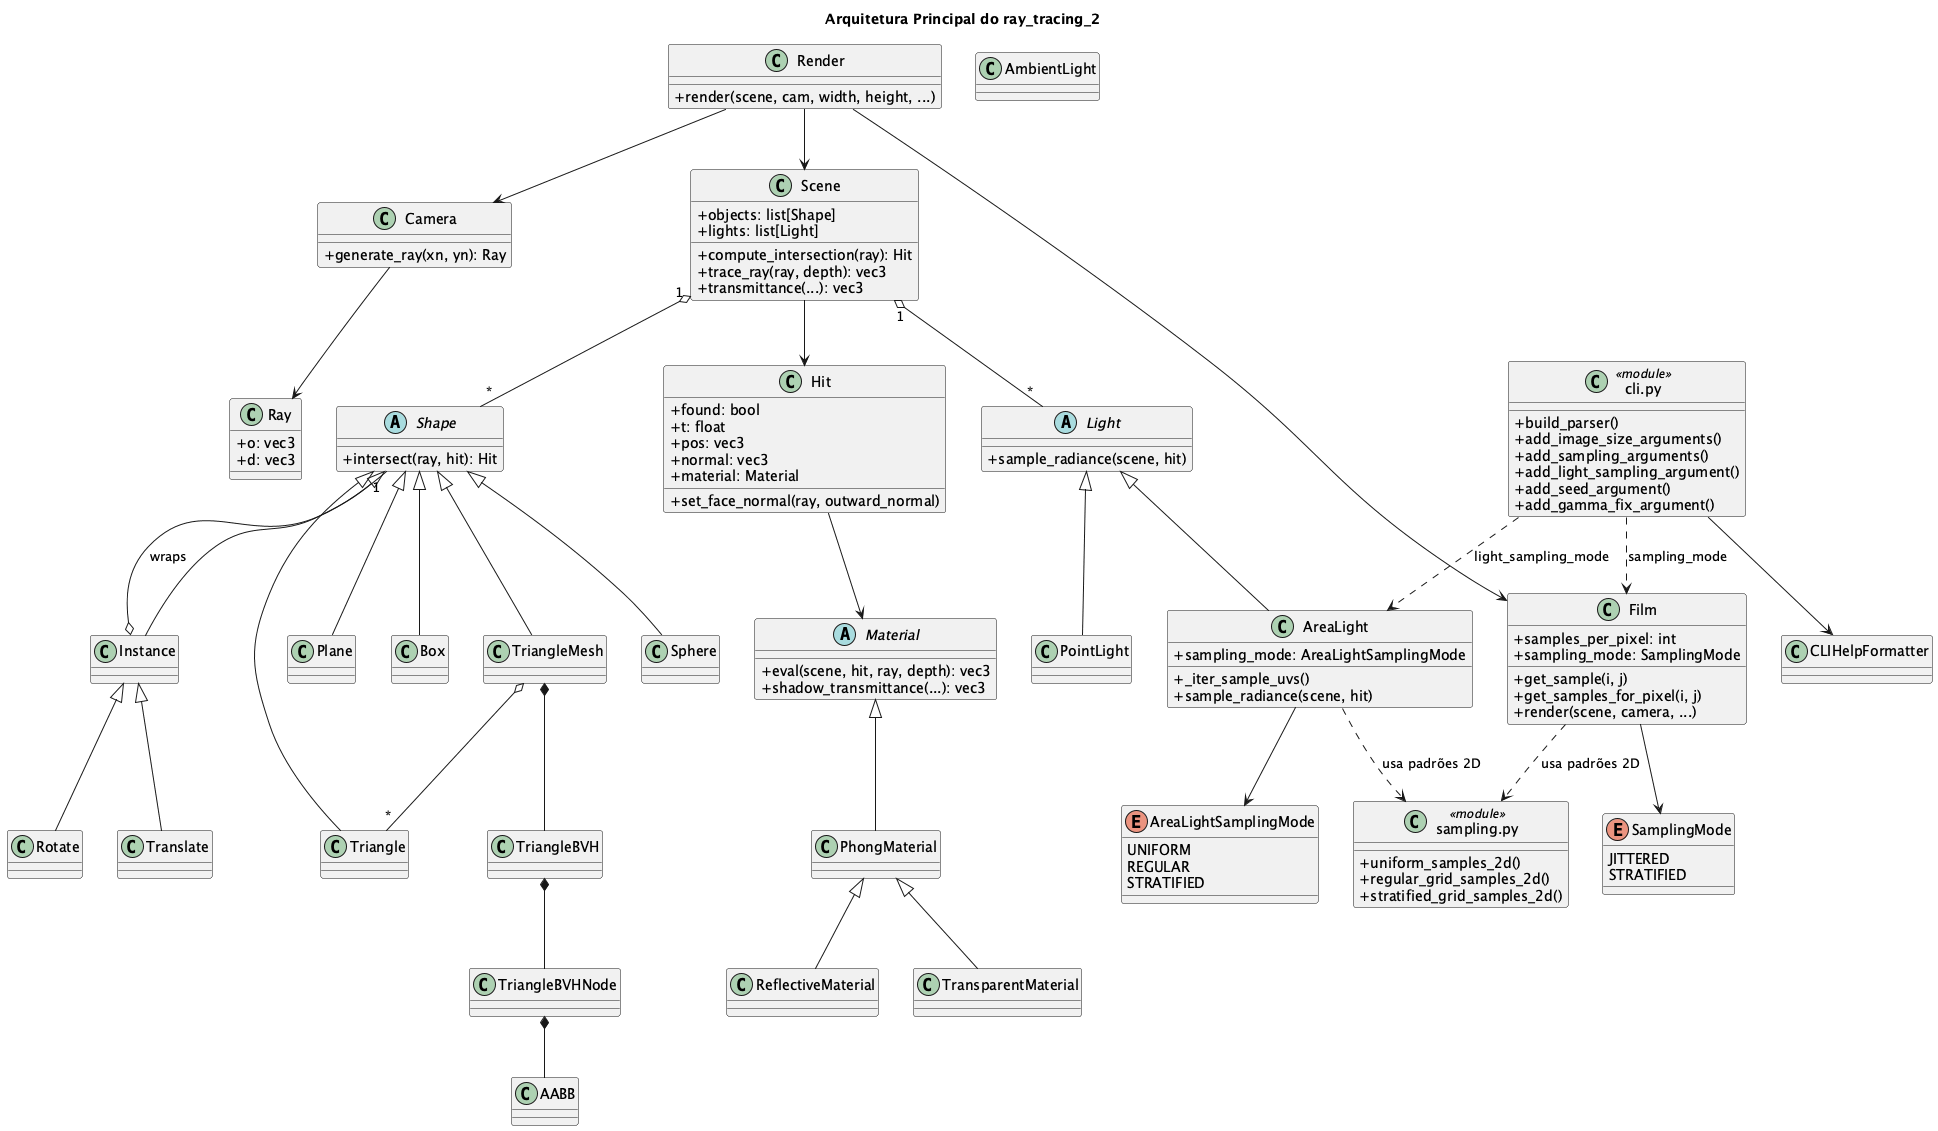
\includegraphics[width=0.95\textwidth]{../ray_tracing_classes_v1.png}
\caption{Versão inicial do diagrama de classes de \texttt{ray\_tracing\_2}, focada no pipeline principal de câmera, filme, cena, materiais, luzes e geometria.}
\label{fig:diagram-class-v1}
\end{figure*}

\subsection*{Versão complementar estendida (v3)}

\begin{figure*}[!ht]
\centering
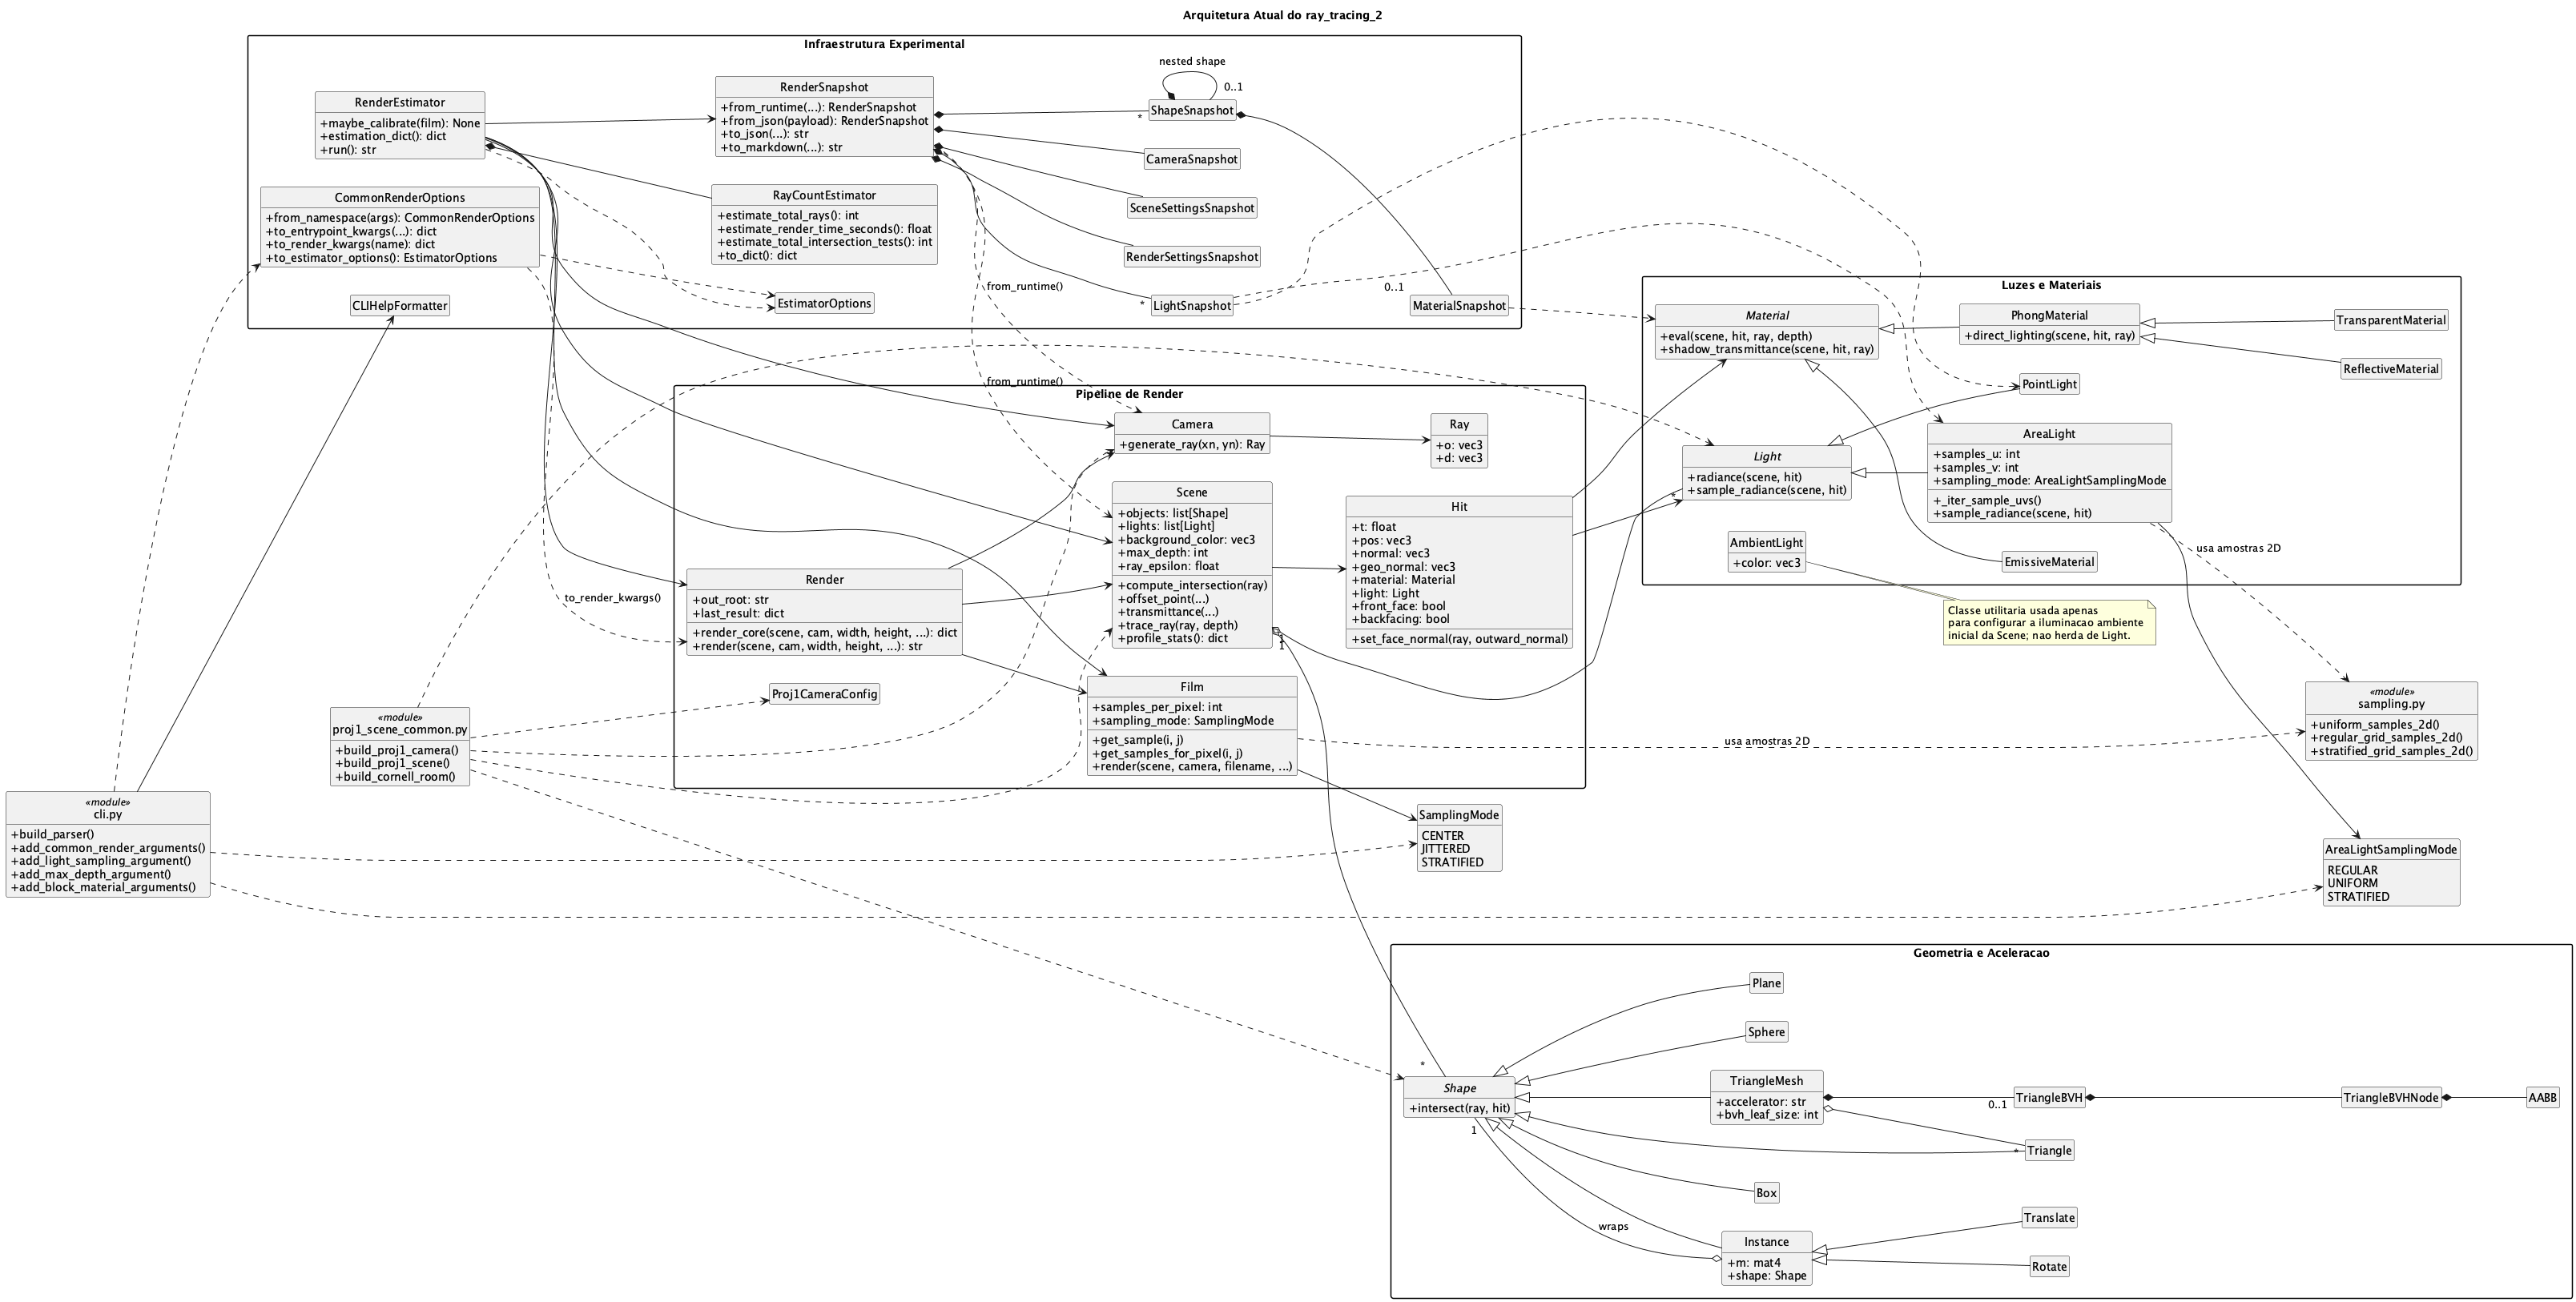
\includegraphics[width=0.95\textwidth]{../ray_tracing_classes_v3.png}
\caption{Versão \texttt{v3} do diagrama de classes de \texttt{ray\_tracing\_2}, adicionando a infraestrutura experimental de CLI, estimativa e snapshots como extensão da leitura inicial.}
\label{fig:diagram-class-v3}
\end{figure*}

\clearpage
\onecolumn
\section*{Anexo C: Galeria Visual Ampliada}

As figuras a seguir reproduzem, em escala ampliada, as principais evidências visuais discutidas no corpo do texto. O objetivo deste anexo é preservar a legibilidade das imagens sem comprometer a diagramação do relatório em duas colunas.

\begin{figure}[!ht]
\centering
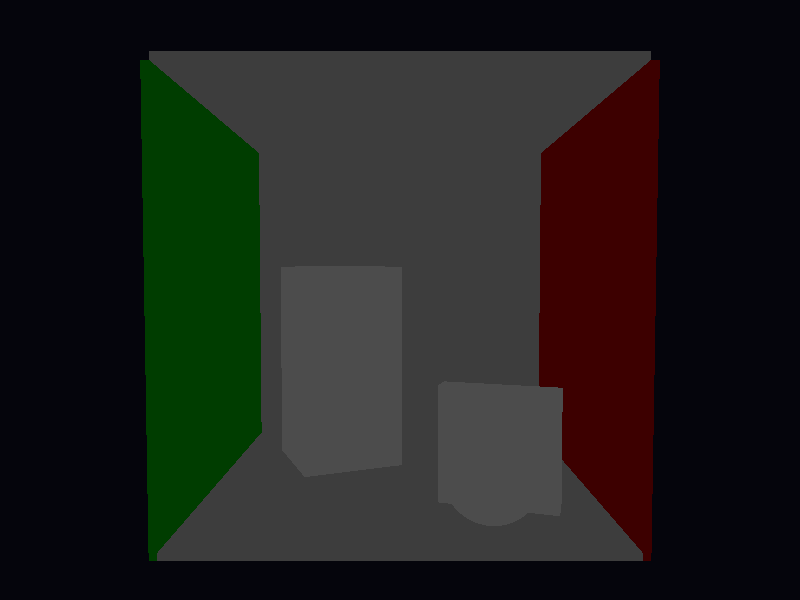
\includegraphics[width=0.92\textwidth]{../outputs/proj1_req1_geometry_20260502_121509/render.png}
\caption{Versão ampliada da Figura~\ref{fig:req1-v3}: geometria e instanciação.}
\end{figure}

\begin{figure}[!ht]
\centering
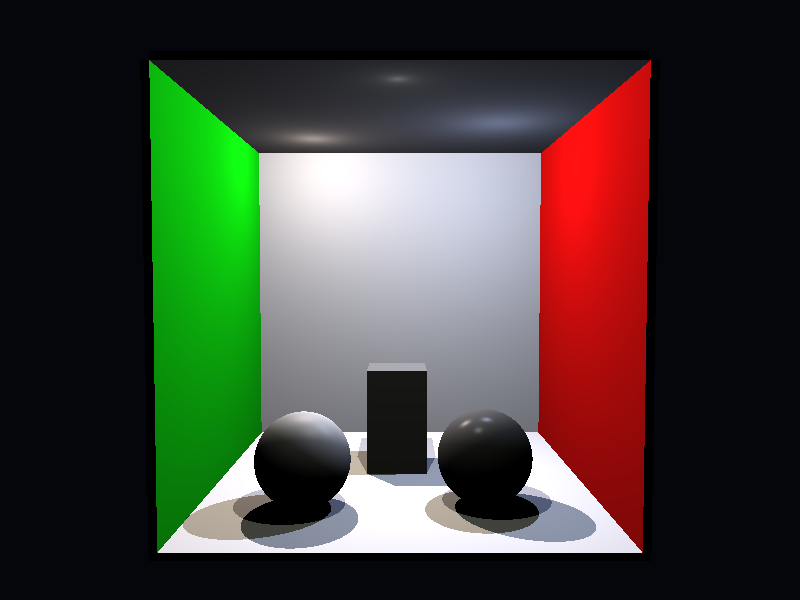
\includegraphics[width=0.92\textwidth]{../outputs/proj1_req2_point_lights_20260502_121731/render.png}
\caption{Versão ampliada da Figura~\ref{fig:req2-v3}: múltiplas fontes pontuais no baseline \texttt{center}.}
\end{figure}

\begin{figure}[!ht]
\centering
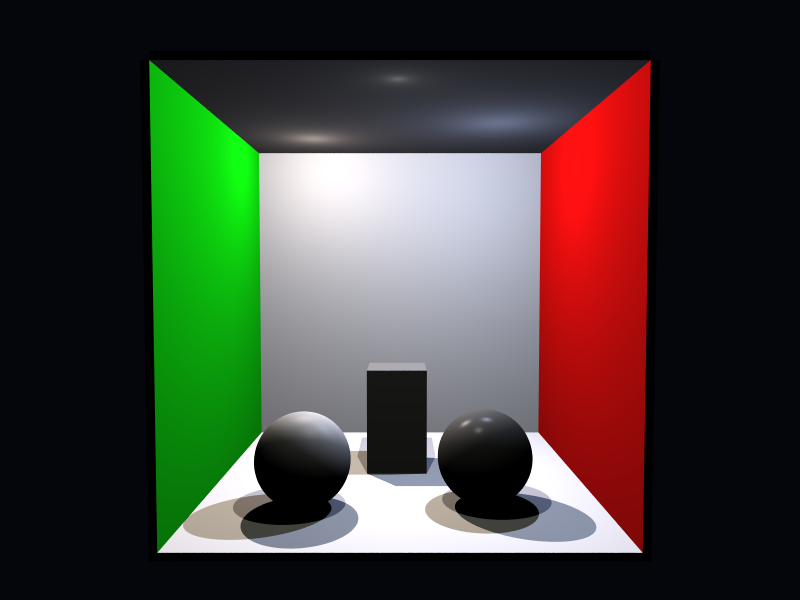
\includegraphics[width=0.92\textwidth]{../outputs/proj1_req2_point_lights_20260502_192411/render.png}
\caption{Versão ampliada da Figura~\ref{fig:req2-aa-v3}: mesma cena com \texttt{stratified} e \(25\) amostras por pixel.}
\end{figure}

\begin{figure}[!ht]
\centering
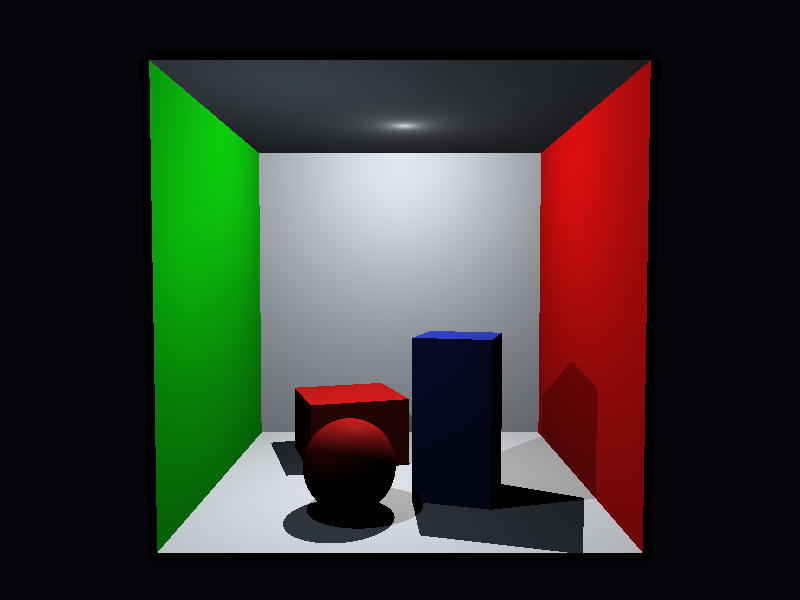
\includegraphics[width=0.92\textwidth]{../outputs/proj1_req3_phong_shadows_20260502_121809/render.png}
\caption{Versão ampliada da Figura~\ref{fig:req3-v3}: Phong com sombras diretas.}
\end{figure}

\begin{figure}[!ht]
\centering
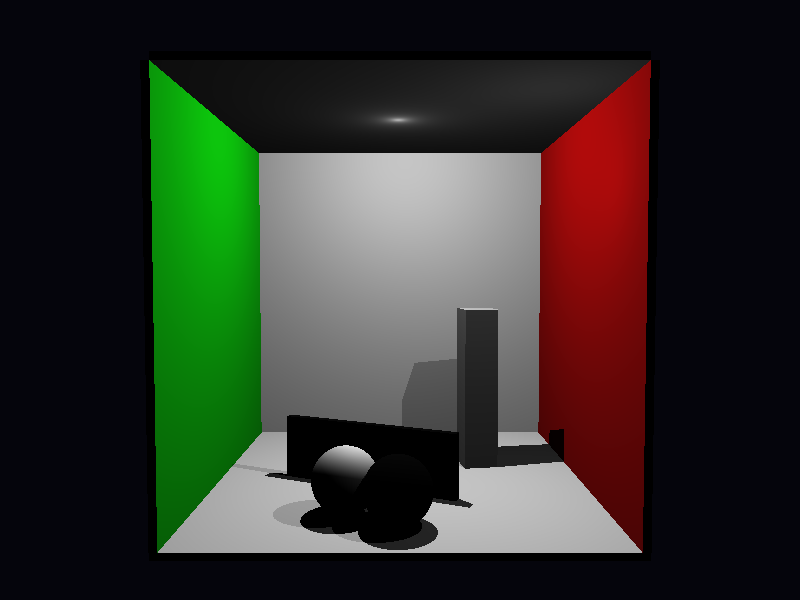
\includegraphics[width=0.92\textwidth]{../outputs/proj1_req4_sampling_20260502_122009/render.png}
\caption{Versão ampliada da Figura~\ref{fig:req4-v3}: baseline \texttt{center} para comparação de antialiasing.}
\end{figure}

\begin{figure}[!ht]
\centering
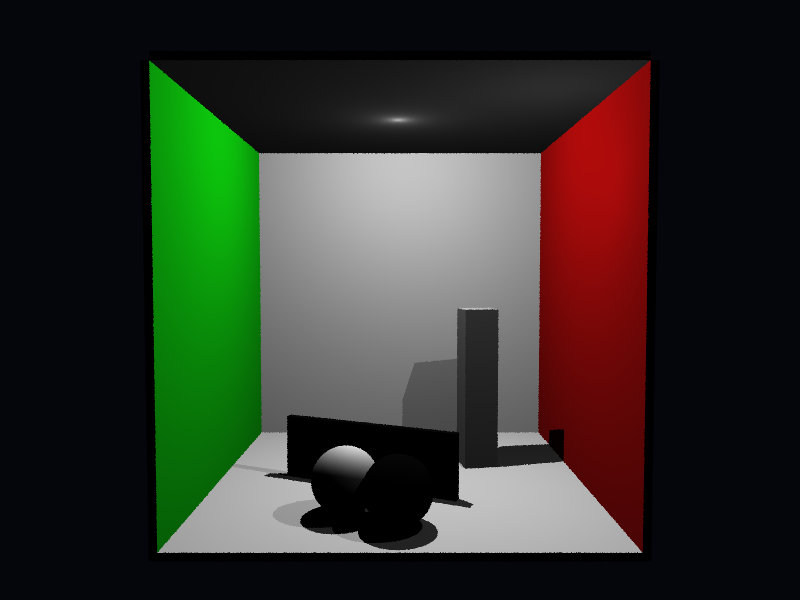
\includegraphics[width=0.92\textwidth]{../outputs/proj1_req4_sampling_20260506_211723/render.png}
\caption{Versão ampliada da Figura~\ref{fig:req4-jittered-v3}: cena de antialiasing com \texttt{jittered}.}
\end{figure}

\begin{figure}[!ht]
\centering
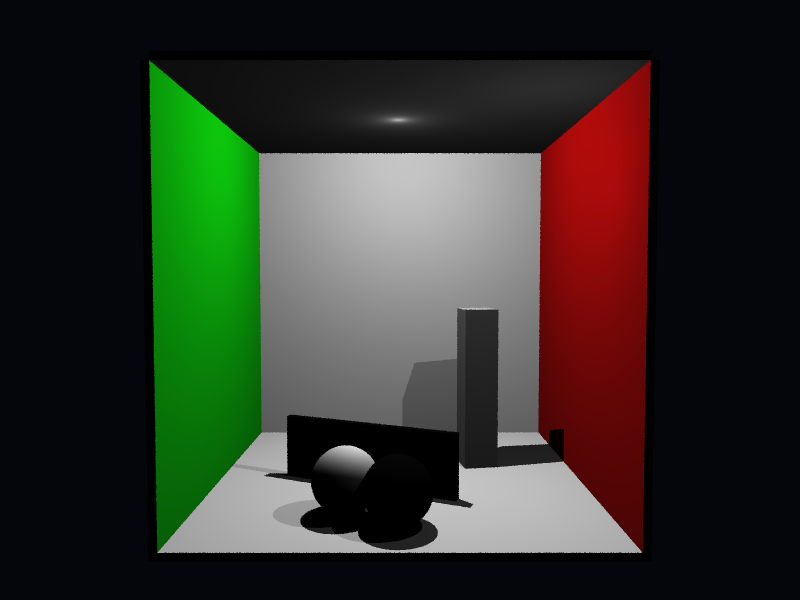
\includegraphics[width=0.92\textwidth]{../outputs/proj1_req4_sampling_20260506_211923/render.png}
\caption{Versão ampliada da Figura~\ref{fig:req4-stratified-v3}: cena de antialiasing com \texttt{stratified}.}
\end{figure}

\begin{figure}[!ht]
\centering
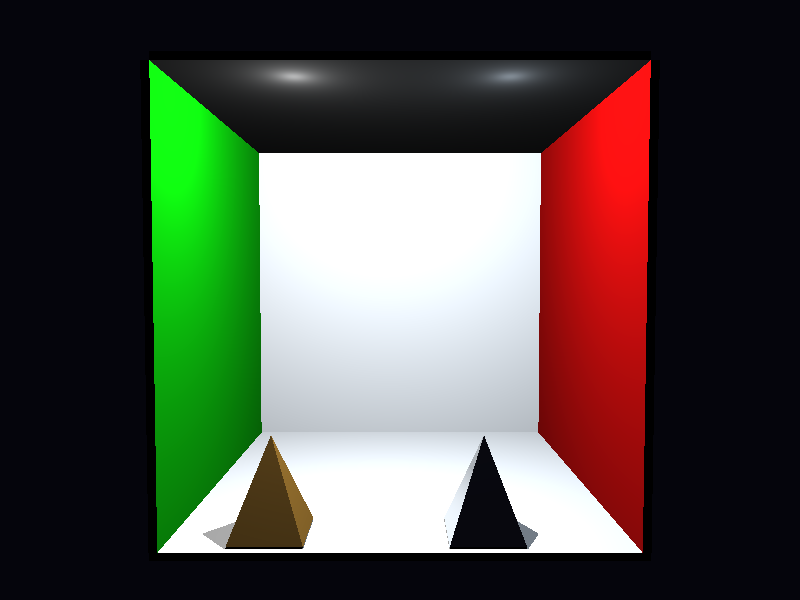
\includegraphics[width=0.92\textwidth]{../outputs/proj1_rext_bvh_20260502_131902/render.png}
\caption{Versão ampliada da Figura~\ref{fig:rext-bvh-v3}: malha triangular com BVH local.}
\end{figure}

\begin{figure}[!ht]
\centering
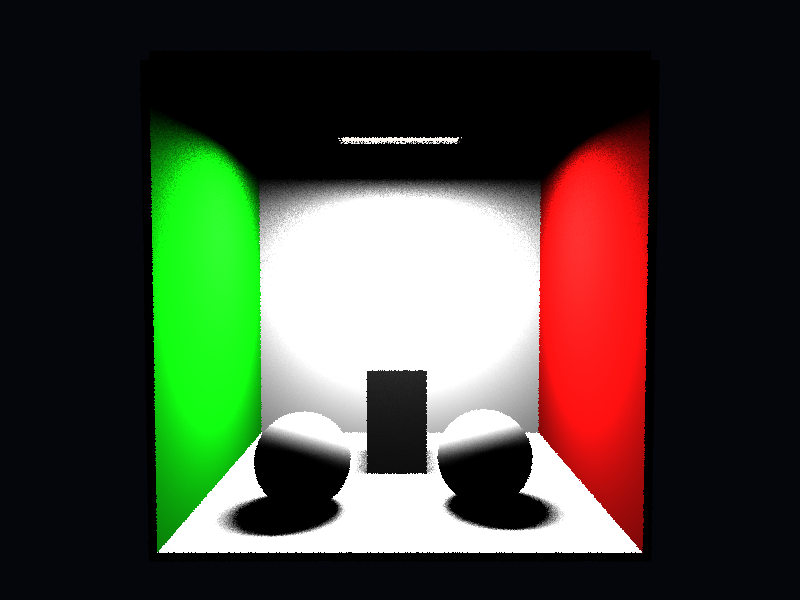
\includegraphics[width=0.92\textwidth]{../outputs/proj1_rext_area_light_20260502_150206/render.png}
\caption{Versão ampliada da Figura~\ref{fig:rext-area-light-v3}: luz de área e emissor visível.}
\end{figure}

\begin{figure}[!ht]
\centering
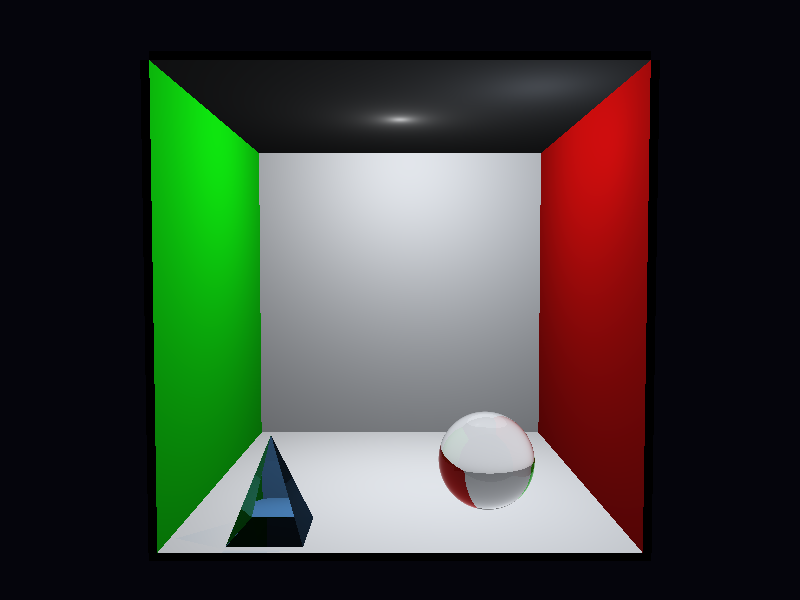
\includegraphics[width=0.92\textwidth]{../outputs/proj1_rext_refractive_20260502_132340/render.png}
\caption{Versão ampliada da Figura~\ref{fig:rext-refractive-v3}: refração, TIR e Beer-Lambert.}
\end{figure}

\begin{figure}[!ht]
\centering
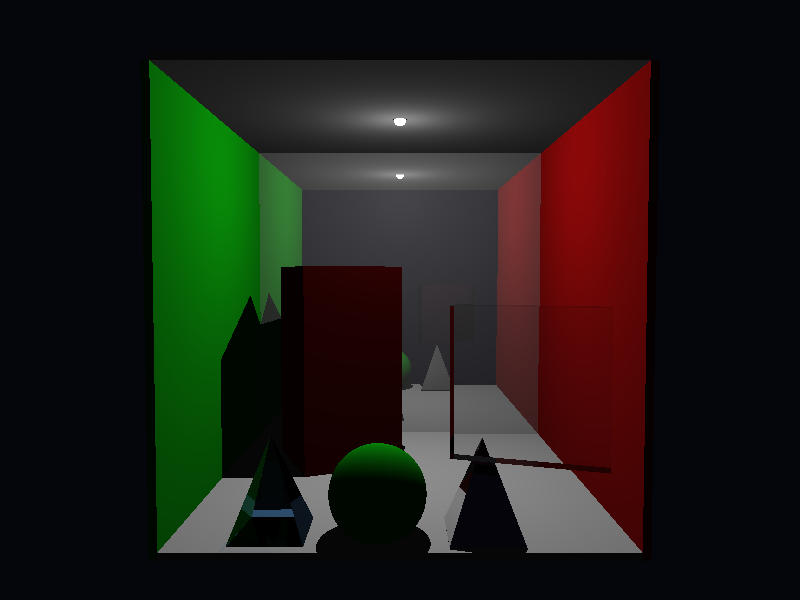
\includegraphics[width=0.92\textwidth]{../outputs/cornell_box_pyramid_20260502_190902/render.png}
\caption{Versão ampliada da Figura~\ref{fig:cornell-center-v3}: cena integrada no baseline \texttt{center}.}
\end{figure}

\begin{figure}[!ht]
\centering
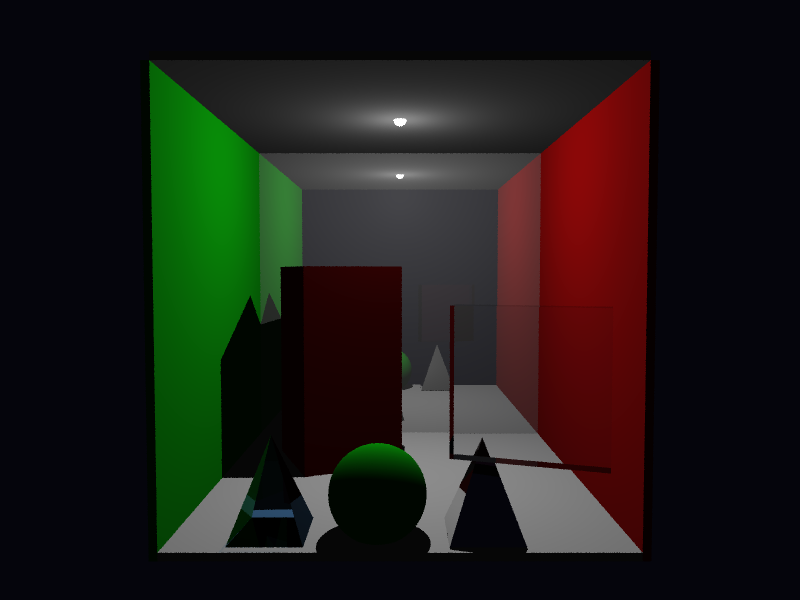
\includegraphics[width=0.92\textwidth]{../outputs/cornell_box_pyramid_20260502_191034/render.png}
\caption{Versão ampliada da Figura~\ref{fig:cornell-stratified-v3}: cena integrada com \texttt{stratified}.}
\end{figure}

\begin{figure}[!ht]
\centering
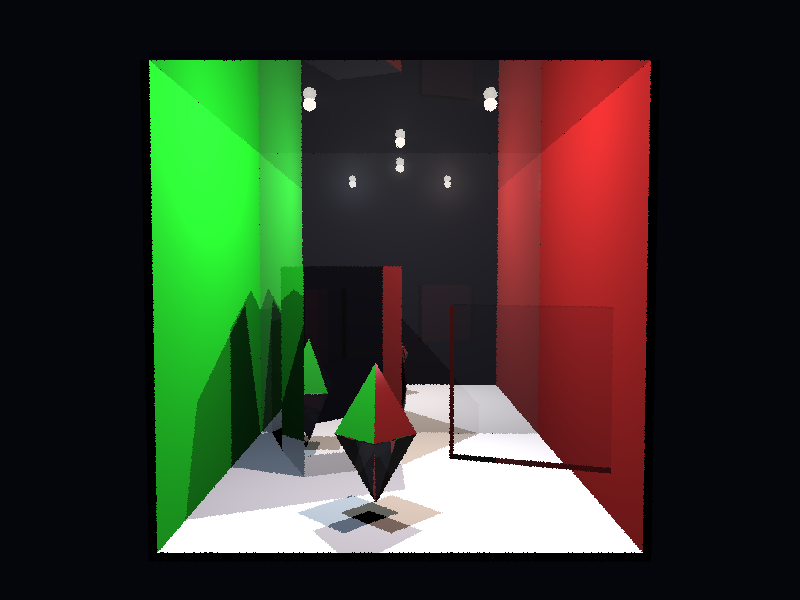
\includegraphics[width=0.92\textwidth]{../outputs/proj1_final_20260502_201946/render.png}
\caption{Versão ampliada da Figura~\ref{fig:proj1-final-v3}: composição final integrada \texttt{proj1\_final}.}
\end{figure}

\begin{figure}[!ht]
\centering
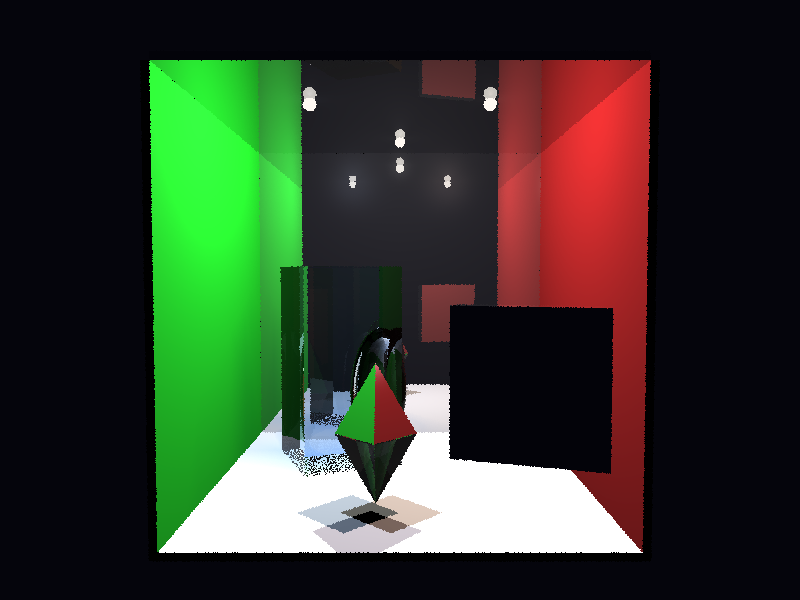
\includegraphics[width=0.92\textwidth]{../outputs/proj1_final_v2_20260502_202707/render.png}
\caption{Versão ampliada da Figura~\ref{fig:proj1-final-v2}: variante integrada \texttt{proj1\_final\_v2}.}
\end{figure}

\begin{figure}[!ht]
\centering
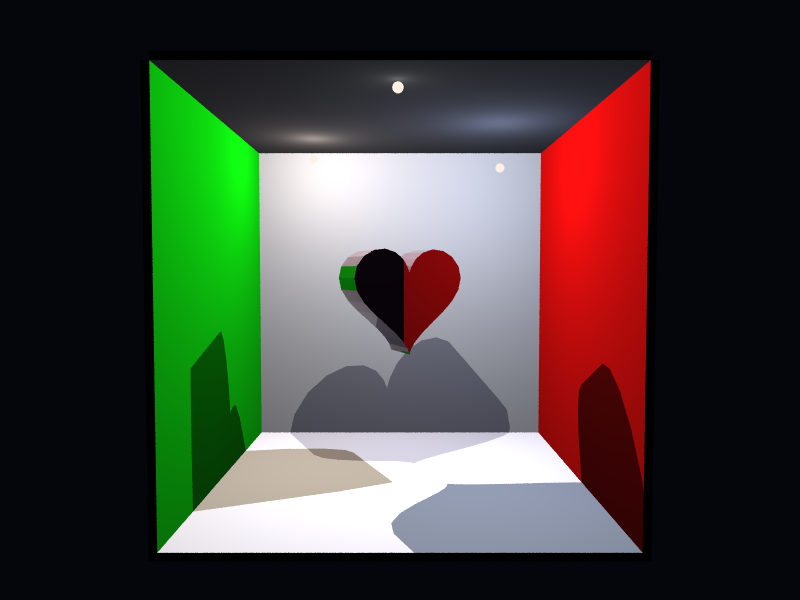
\includegraphics[width=0.92\textwidth]{../outputs/proj1_heart_trianglemesh_20260502_205136/render.png}
\caption{Versão ampliada da Figura~\ref{fig:heart-triangle-v3}: malha cardíaca triangulada com \texttt{bvh}.}
\end{figure}

\subsection*{Exemplos exploratórios recuperados por snapshot}

As figuras a seguir reúnem artefatos exploratórios anexados pelo autor e preservados pelas saídas \texttt{properties.md}/\texttt{properties.json}. Elas complementam o corpo do texto ao mostrar como a camada de snapshots permite recuperar cenas intermediárias e variações de modelagem que não entraram na espinha principal do relatório, mas continuam úteis como evidência de exploração técnica.

\begin{figure}[!ht]
\centering
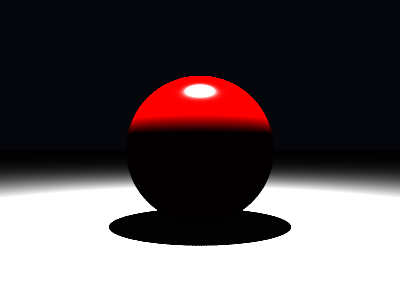
\includegraphics[width=0.92\textwidth]{../outputs/main_scene_20260405_171334/render.png}
\caption{Artefato inicial de \texttt{main\_scene}: cena mínima com esfera sobre plano e \texttt{properties.md} em formato explicativo.}
\end{figure}

\begin{figure}[!ht]
\centering
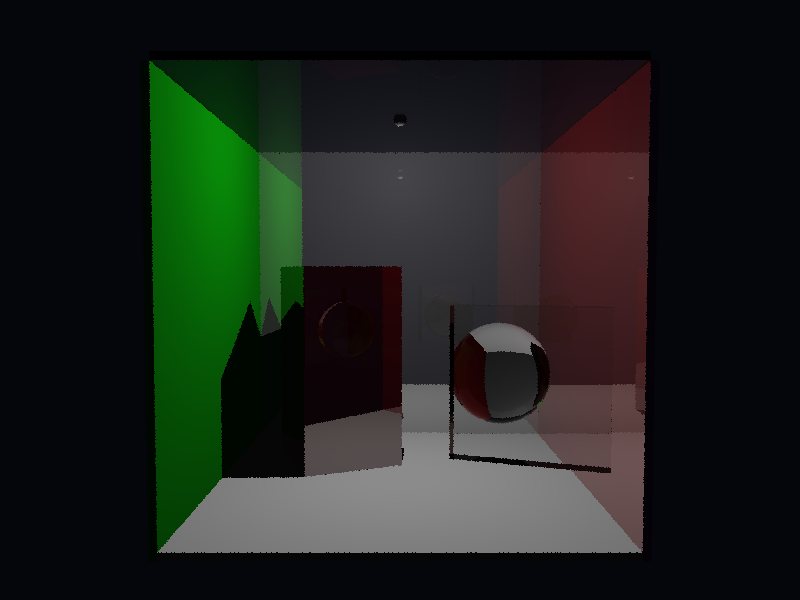
\includegraphics[width=0.92\textwidth]{../outputs/cornell_box_20260412_233524/render.png}
\caption{Variação exploratória de \texttt{cornell\_box}: esfera transparente frontal e composição interna preservadas por snapshot.}
\end{figure}

\begin{figure}[!ht]
\centering
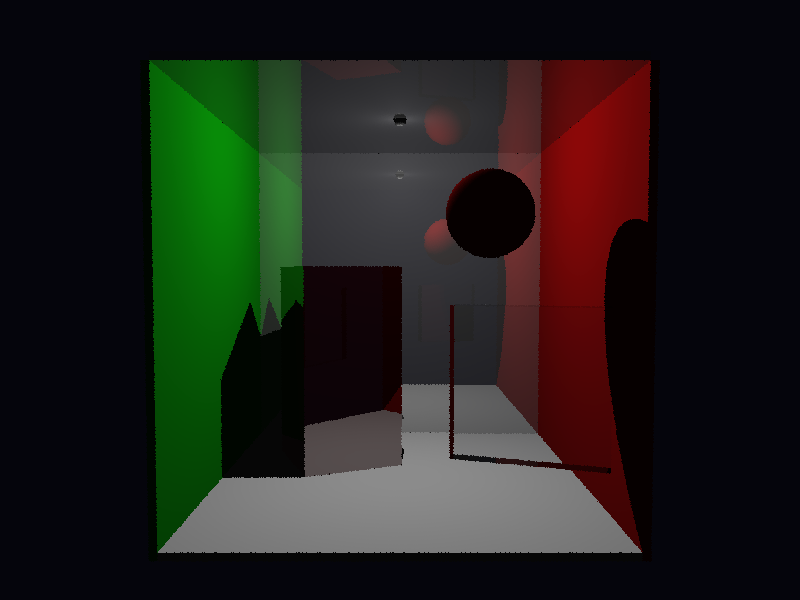
\includegraphics[width=0.92\textwidth]{../outputs/cornell_box_20260412_233959/render.png}
\caption{Outra variação de \texttt{cornell\_box}: esfera refletiva em destaque e plano transparente interno.}
\end{figure}

\begin{figure}[!ht]
\centering
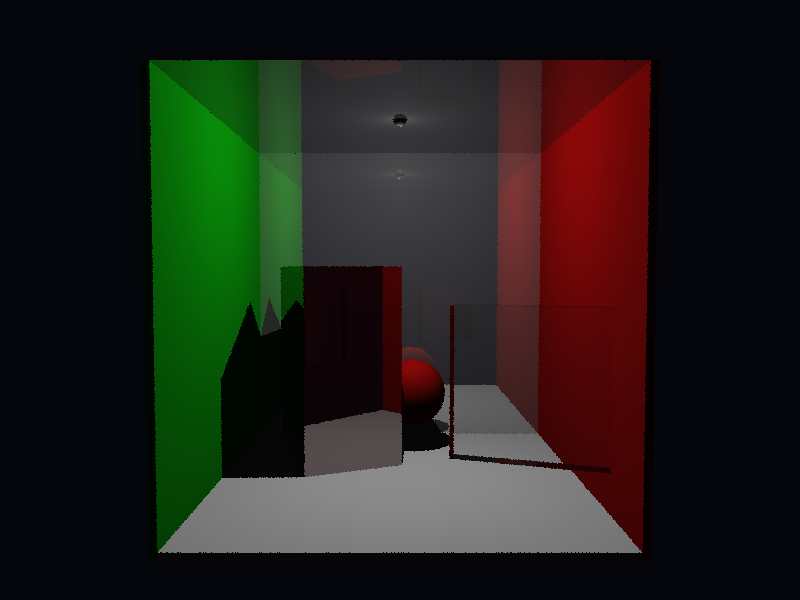
\includegraphics[width=0.92\textwidth]{../outputs/cornell_box_20260412_234221/render.png}
\caption{Variação de \texttt{cornell\_box} com esfera vermelha deslocada para a região frontal da cena.}
\end{figure}

\begin{figure}[!ht]
\centering
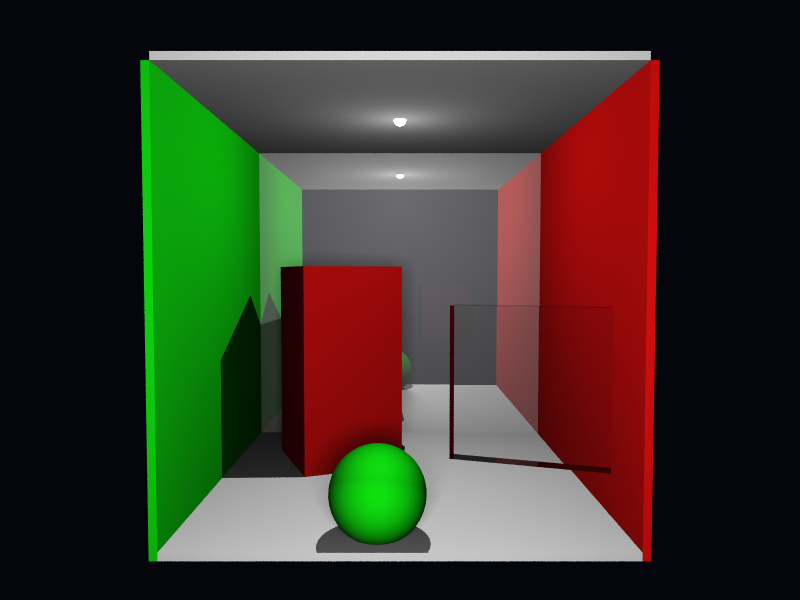
\includegraphics[width=0.92\textwidth]{../outputs/cornell_box_20260413_195851/render.png}
\caption{Variação de \texttt{cornell\_box} com \(25\) amostras em \texttt{jittered} e múltiplas luzes pontuais.}
\end{figure}

\begin{figure}[!ht]
\centering
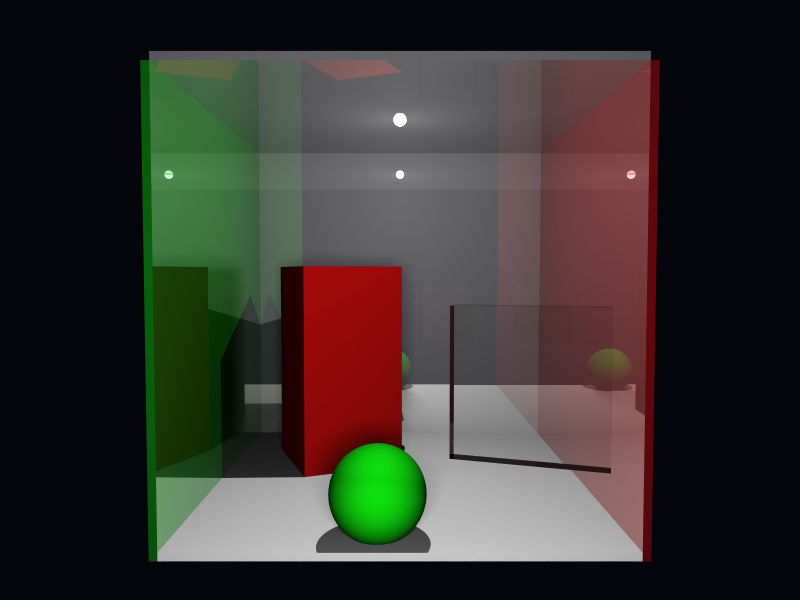
\includegraphics[width=0.92\textwidth]{../outputs/cornell_box_20260413_214356/render.png}
\caption{Variação de \texttt{cornell\_box} com \(25\) amostras em \texttt{stratified} e paredes refletivas.}
\end{figure}

\begin{figure}[!ht]
\centering
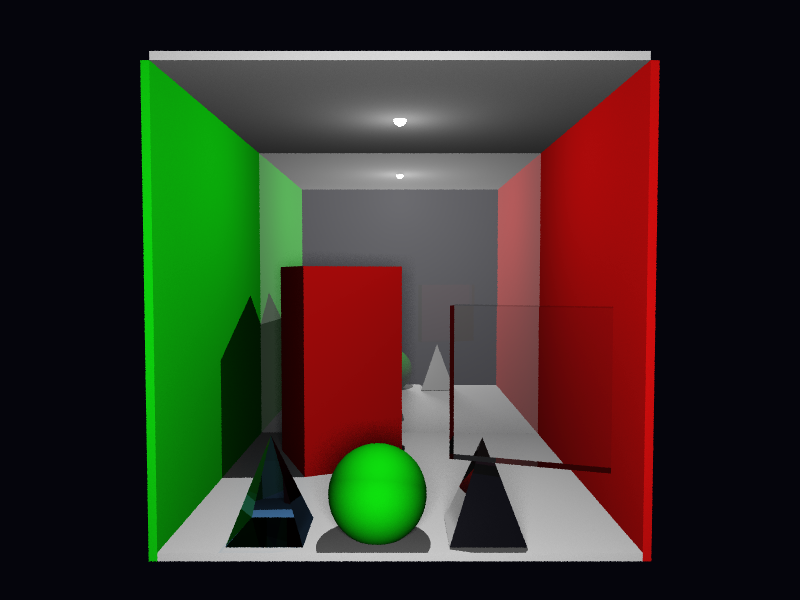
\includegraphics[width=0.92\textwidth]{../outputs/cornell_box_pyramid_20260501_214225/render.png}
\caption{Variação adicional de \texttt{cornell\_box\_pyramid}: \(10\) amostras em \texttt{jittered}, malhas triangulares e luz de área estratificada.}
\end{figure}

\end{document}